% !TeX program = xelatex
%% % !TEX TS-program = xelatex

%-------------------------------------------------------------
% Preamble
%-------------------------------------------------------------
\documentclass[12pt, aspectratio=169, xcolor=dvipsnames]{beamer}
%\documentclass[12pt,aspectratio=169,xcolor=dvipsnames,handout,notes=show]{beamer}	  % For printing
%% Packages for Beamer
% Conditionals, Fromatting, Lists, Figures, Tables, Math,
% Hyperlinks and References, Special Characters, Theme

%---------------------------------------------------------------
% Conditionals
%---------------------------------------------------------------
\usepackage{etoolbox}						% For conditionals (e.g. slides with stops)
	\providetoggle{long}					   % Generates long vs. short version
	\settoggle{long}{false} 					% 'false' for version without stops

	\providetoggle{struct}					   % Generates long vs. short version
	\settoggle{struct}{false}					% 'true' for version with customized stops

%---------------------------------------------------------------
% Fromatting
%---------------------------------------------------------------
\setbeamertemplate{navigation symbols}{}				% Omits the navigation symbols
\usepackage{todonotes} 											  % Used for to-do lists
\usepackage{setspace} 		% Line spacing and spaces above/below equations
	\setstretch{1.7}
	\AtBeginDocument{		 % Space before and after an equation
		\addtolength\abovedisplayskip{-0.5\baselineskip}
		\addtolength\belowdisplayskip{-0.5\baselineskip}}

%---------------------------------------------------------------
% Lists
%---------------------------------------------------------------
\usepackage{enumerate} 											% Personalizes the enumerate style
	\setbeamertemplate{enumerate items}[default]
	\setbeamertemplate{itemize items}{$\bullet$}		 % Or {$\vdash$}
	\setbeamertemplate{itemize subitem}{$\rightharpoonup$}
	\setbeamertemplate{itemize subsubitem}{---}
	%\setbeamertemplate{itemize subsubitem}[triangle]
	%\setbeamercolor{subitem projected}{bg=green}
	%\setbeamercolor{itemize subitem}{bg=green}
%\usepackage[orientation=landscape,size=custom,width=16,height=9.75,scale=0.5,debug]{beamerposter}

%---------------------------------------------------------------
% Figures
%---------------------------------------------------------------
\usepackage{tikz}								% To create high quality diagrams
\usepackage{graphicx} 				 		% Needed for \includegraphics
\usepackage[outdir=./]{epstopdf} 	  % Avoids errors to input figures
%\usepackage[texcoord,grid,gridunit=mm,gridcolor=red!10,subgridcolor=green!10]
%{eso-pic}											 % Draw grid on slide to aid positioning figures

%---------------------------------------------------------------
% Tables
%---------------------------------------------------------------
\usepackage{booktabs}						% Needed for \toprule, \midrule, \bottomrule

%---------------------------------------------------------------
% Math
%---------------------------------------------------------------
\usepackage{amsmath} 					  % Needed for command eqref
\usepackage{amssymb} 					 % Needed for math fonts
%\usepackage{breqn}						    % Break lines automatically
%\usepackage{amssymb,amsmath,amsthm,enumitem}

%---------------------------------------------------------------
% Hyperlinks and References
%---------------------------------------------------------------
\usepackage[absolute,overlay]{textpos}	% Positioning text in slide (e.g. links to slides)
\usepackage{hyperref}				  % For hyperlinks, [colorlinks=true] gets rid of the awful boxes
\usepackage{xcolor}
	\definecolor{c1}{rgb}{0,0,1} 		  % Blue
	\definecolor{c2}{rgb}{0,0.3,0.9} 	% Light blue
	\definecolor{c3}{rgb}{0.3,0,0.9} 	% Red blue
	\hypersetup{
		linkcolor={c1}, 						% Internal links
		citecolor={c2}, 						% Citations
		urlcolor={c3} 							 % External links/urls
	}
\usepackage[round,authoryear]{natbib} % For cite and abbrvnat bibliography style
%\usepackage{cite} 							% Needed for cite

%---------------------------------------------------------------
% Special Characters
%---------------------------------------------------------------
\usepackage[utf8]{inputenc}			  % Input accented characters
%\usepackage{underscore}				   % Control the behaviour of "_" in the text
%\usepackage[T1]{fontenc}		  	  % Fonts to use for printing characters

%---------------------------------------------------------------
% Theme
%---------------------------------------------------------------
\usetheme{Madrid}			   % Good: Madrid, Copenhagen, CambridgeUS, Boadilla
\useoutertheme{noslidenum}
\usecolortheme{lily} 			% Good: lily, dolphin
\usefonttheme{serif}
\useoutertheme{infolines} 	% Full list: miniframes, infolines, shadow, sidebar, smoothbars, smoothtree, split, tree
%\useinnertheme{circles}	 % Full list: rectangles, circles, inmargin, rounded
\definecolor{JHUblue}{rgb}{0.36, 0.54, 0.66}%{0, 0.45, 0.114}
\definecolor{JHUgrey2}{rgb}{180, 178, 173}
\definecolor{JHUorange}{rgb}{255, 105, 0}
\definecolor{airforceblue}{rgb}{0.36, 0.54, 0.66}
\definecolor{bluegray}{rgb}{0.4, 0.6, 0.8}
\definecolor{cerulean}{rgb}{0.0, 0.48, 0.65}
\definecolor{darkcerulean}{rgb}{0.03, 0.27, 0.49}
\definecolor{darkpastelblue}{rgb}{0.47, 0.62, 0.8}
\definecolor{glaucous}{rgb}{0.38, 0.51, 0.71}
\definecolor{hanblue}{rgb}{0.27, 0.42, 0.81}
\definecolor{iceberg}{rgb}{0.44, 0.65, 0.82}
\definecolor{indigo}{rgb}{0.0, 0.25, 0.42}		% with infolines
\definecolor{internationalkleinblue}{rgb}{0.0, 0.18, 0.65}
\definecolor{lapislazuli}{rgb}{0.15, 0.38, 0.61}
\definecolor{mediumelectricblue}{rgb}{0.01, 0.31, 0.59}  %Good
\definecolor{mediumpersianblue}{rgb}{0.0, 0.4, 0.65}
\definecolor{mediumtealblue}{rgb}{0.0, 0.33, 0.71}
\definecolor{midnightblue}{rgb}{0.1, 0.1, 0.44}		% Cool dark
\definecolor{navyblue}{rgb}{0.0, 0.0, 0.5}		% Darker than standard purple
\definecolor{phthaloblue}{rgb}{0.0, 0.06, 0.54}
\definecolor{smalt}{rgb}{0.0, 0.2, 0.6} 		% Nice close to standard
\definecolor{oceanboatblue}{rgb}{0.0, 0.47, 0.75}  % Blue green
\definecolor{steelblue}{rgb}{0.27, 0.51, 0.71}
\definecolor{oucrimsonred}{rgb}{0.6, 0.0, 0.0}  % Brick red
\definecolor{pansypurple}{rgb}{0.47, 0.09, 0.29}
\definecolor{palatinatepurple}{rgb}{0.41, 0.16, 0.38} % Purple brownish
\definecolor{parisgreen}{rgb}{0.31, 0.78, 0.47}
\definecolor{seagreen}{rgb}{0.18, 0.55, 0.34}
\definecolor{skobeloff}{rgb}{0.0, 0.48, 0.45}	% Elegant green
\definecolor{pastelblue}{rgb}{0.68, 0.78, 0.81}  % Grey with contrast
\definecolor{redncs}{rgb}{0.77, 0.01, 0.2}
\definecolor{richcarmine}{rgb}{0.84, 0.0, 0.25}
\definecolor{royalazure}{rgb}{0.0, 0.22, 0.66}
\definecolor{royalblue}{rgb}{0.0, 0.14, 0.4}	% Almost black
\definecolor{stpatricksblue}{rgb}{0.14, 0.16, 0.48}		% Darkish blue
\definecolor{sapphire}{rgb}{0.03, 0.15, 0.4}	% Elegant darkish blue
\definecolor{tuftsblue}{rgb}{0.28, 0.57, 0.81} 	% Fresh light blue-green
\definecolor{unitednationsblue}{rgb}{0.36, 0.57, 0.9}
\definecolor{yaleblue}{rgb}{0.06, 0.3, 0.57}	% Good

\usecolortheme[named=yaleblue]{structure}
\setbeamercolor{alerted text}{fg=midnightblue}
\setbeamerfont{alerted text}{series=\bfseries}

%---------------------------------------------------------------
% Sources
%---------------------------------------------------------------
% http://latexcolor.com/
% https://ramblingacademic.com/2015/12/how-to-quickly-overhaul-beamer-colors/

% Position text in a slide
%https://tex.stackexchange.com/questions/82463/how-to-position-a-beamer-box-in-a-slide

% To draw a box above a table (stored as an image)
%https://www.overleaf.com/learn/latex/LaTeX_Graphics_using_TikZ:_A_Tutorial_for_Beginners_(Part_1)%E2%80%94Basic_Drawing
%https://tex.stackexchange.com/questions/115087/how-can-i-embed-an-external-image-within-a-tikzpicture-environment
%https://tex.stackexchange.com/questions/57913/putting-a-box-over-an-image-in-beamer-presentation   		  % Packages
%% Personalized Macros
% Definitions, Equations, Table of Contents, Tables, Subcaptions, Paths, Text Fomats

%-------------------------------------------------------------------
% Variable Definitions
%-------------------------------------------------------------------
\providecommand{\tnr}{n}
\providecommand{\tnrfwd}{m}
\providecommand{\idxt}{t}
\providecommand{\idxi}{i}
\providecommand{\idxh}{h}
\providecommand{\idxs}{\idxt,\tnr}
\providecommand{\idxsfwd}{\tnr | \tnrfwd}
\providecommand{\idxsfwdt}{\idxt,\idxsfwd}
\providecommand{\idxspnl}{\idxi,\idxt}
\providecommand{\idxspnlfwd}{\idxi,{\idxt+\idxh}}
\providecommand{\idxspnllag}{\idxi,{\idxt-1}}
\providecommand{\idxspnllaglag}{\idxi,{\idxt-j}}
\providecommand{\fInst}{f_{\idxs}}
\providecommand{\yld}{y}
\providecommand{\xpc}{e}
\providecommand{\yZero}{\yld_{\idxs}}
\providecommand{\yZeroQ}{\yZero^{\Qmeasure}}
\providecommand{\yZeroP}{\yZero^{\Pmeasure}}
\providecommand{\yZeroE}{\yZero^{\xpc}}
\providecommand{\yZeroFwd}{\frate_{\idxsfwdt}}
\providecommand{\yZeroEfwd}{\yZeroFwd^{\xpc}}
\providecommand{\Pzero}{P_{\idxs}}
\providecommand{\Pzerolag}{P_{\idxt+1,\tnr-1}}
\providecommand{\srate}{i}
\providecommand{\shortrate}{\srate_{\idxt}}
\providecommand{\shortratelag}{\srate_{\idxt-1}}
\providecommand{\frate}{f}
\providecommand{\realrate}{r_{\idxs}}
\providecommand{\rateSvy}{\srate_{\idxs}^{survey}}
\providecommand{\SDF}{M_{\idxt+1}}
\providecommand{\SDFprod}{\ExpP \left[\Pi_{j=1} ^\tnr M_{\idxt+j}\right]}
\providecommand{\SDFsum}{\ExpQ \left[\exp \left(- \Sigma_{j=0} ^{\tnr-1} \srate_{\idxt+j} \right) \right]}
\providecommand{\Xvars}{X_{\idxt}}
\providecommand{\XvarsFwd}{X_{\idxt+1}}
\providecommand{\affineA}{A_{\tnr}}
\providecommand{\affineB}{B_{\tnr}}
\providecommand{\affineAfwd}{A_{\tnr + 1}}
\providecommand{\affineBfwd}{B_{\tnr + 1}}
\providecommand{\affineAQ}{\affineA^{\Qmeasure}}
\providecommand{\affineBQ}{\affineB^{\Qmeasure}}
\providecommand{\affineAP}{\affineA^{\Pmeasure}}
\providecommand{\affineBP}{\affineB^{\Pmeasure}}
\providecommand{\affineAe}{\affineA^{\xpc}}
\providecommand{\affineBe}{\affineB^{\xpc}}
\providecommand{\affineAeFwd}{A_{\idxsfwd}^{\xpc}}
\providecommand{\affineBeFwd}{B_{\idxsfwd}^{\xpc}}
\providecommand{\yLCnom}{\yld_{\idxs} ^{LC}}
\providecommand{\yLCsynt}{\widetilde{\yld}_{\idxs} ^{LC}}
\providecommand{\yUS}{y_{\idxs} ^{US}}
\providecommand{\yUSsynt}{\widetilde{\yld}_{\idxs} ^{US}}
\providecommand{\fx}{\mathit{s}}

% Math fonts
\providecommand{\Xdim}{\mathrm{K}}
\providecommand{\Ydim}{\mathrm{N}}
\providecommand{\Sdim}{\mathrm{S}}
\providecommand{\Normal}{\mathcal{N}}
\providecommand{\Pmeasure}{\mathbb{P}}
\providecommand{\Qmeasure}{\mathbb{Q}}
\providecommand{\Expec}{\mathrm{E}_{t}}
\providecommand{\ExpP}{\mathrm{E}^{\Pmeasure}_{t}}
\providecommand{\ExpQ}{\mathrm{E}^{\Qmeasure}_{t}}
\providecommand{\Svy}{S}
\providecommand{\yVec}{\mathbf{\yld}_{t}}
\providecommand{\ySVec}{\yVec^{\Svy}}
\providecommand{\Avec}{\mathbf{A}}
\providecommand{\Bvec}{\mathbf{B}}
\providecommand{\ASvec}{\mathbf{A}^{\Svy}}
\providecommand{\BSvec}{\mathbf{B}^{\Svy}}
\providecommand{\uVec}{\mathbf{u}_{t}}
\providecommand{\uSVec}{\mathbf{u}_{t}^{\Svy}}
\providecommand{\Svec}{\mathbf{\Sigma}}
\providecommand{\SyVec}{\mathbf{\Svec}_{Y}}
\providecommand{\SsVec}{\mathbf{\Svec}_{\Svy}}

% Greeks
\providecommand{\termprm}{\tau_{\idxs}}
\providecommand{\riskprice}{\lambda_{t}}
\providecommand{\lambdazero}{\lambda_{0}}
\providecommand{\lambdaone}{\lambda_{1}}
\providecommand{\fwdprm}{\rho_{\idxs}}
\providecommand{\CIPdev}{\phi_{\idxs}}
\providecommand{\deltazero}{\delta_{0}}
\providecommand{\deltaone}{\delta_{1}}
\providecommand{\error}{\nu_{t+1}}
\providecommand{\errorQ}{\error^{\Qmeasure}}
\providecommand{\errorP}{\error^{\Pmeasure}}
\providecommand{\XmuP}{\mu^{\Pmeasure}}
\providecommand{\XmuQ}{\mu^{\Qmeasure}}
\providecommand{\XSigma}{\Sigma}
\providecommand{\XPhiP}{\Phi^{\Pmeasure}}
\providecommand{\XPhiQ}{\Phi^{\Qmeasure}}
\providecommand{\betaLT}{\beta_{0}}
\providecommand{\betaST}{\beta_{1}}
\providecommand{\betaMTns}{\beta_{2}}
\providecommand{\betaMTnss}{\beta_{3}}
\providecommand{\tauNS}{\tau_{1}}
\providecommand{\tauNSS}{\tau_{2}}
\providecommand{\tnrTauNS}{\tnr/\tauNS}
\providecommand{\tnrTauNSS}{\tnr/\tauNSS}
\providecommand{\params}{\theta}
\providecommand{\Vasy}{\Omega}
\providecommand{\cmpnt}{\Psi}
\providecommand{\Jacobian}{\Gamma}
\providecommand{\Hessian}{\mathcal{H}_\params}
\providecommand{\asydstr}{\sqrt{\Ydim} \left( \widehat{\cmpnt} - \cmpnt \right) \xrightarrow[]{d} \Normal \left(0,\, \Jacobian \, \Vasy \, \Jacobian' \right)}
\providecommand{\sampleHjoint}{\frac{1}{\Ydim} \frac{\partial^{2} \ell_{\Ydim} (\widehat{\params})}{\partial \params \partial \params'}}
\providecommand{\sampleHindiv}{\frac{1}{\Ydim} \sum_{i = 1}^{\Ydim} \frac{\partial^{2} \log \mathit{f} (X_{i} | \widehat{\params})}{\partial \params \partial \params'}}

% Nelson-Siegel_Svensson
\providecommand{\loadSTnsFwd}{\exp\left(-\tnrTauNS \right)}
\providecommand{\loadSTnssFwd}{\exp\left(-\tnrTauNSS \right)}
\providecommand{\loadMTnsFwd}{\left(\tnrTauNS\right) \loadSTnsFwd}
\providecommand{\loadMTnssFwd}{\left(\tnrTauNSS\right) \loadSTnssFwd}
\providecommand{\loadSTnsZero}{\frac{1-\loadSTnsFwd}{\tnrTauNS}}
\providecommand{\loadSTnssZero}{\frac{1-\loadSTnssFwd}{\tnrTauNSS}}
\providecommand{\loadMTnsZero}{\left(\loadSTnsZero - \loadSTnsFwd \right)}
\providecommand{\loadMTnssZero}{\left( \loadSTnssZero - \loadSTnssFwd \right)}

%\providecommand{\}{}
% DELETE in a later revision
\providecommand{\Xmu}{\mu}
\providecommand{\XPhi}{\Phi}
\providecommand{\XmuStar}{\mu^{*}}
\providecommand{\XPhiStar}{\Phi^{*}}
\providecommand{\STrate}{r}
\providecommand{\rShort}{\STrate_{t}}
\providecommand{\rShortlag}{\STrate_{t-1}}
\providecommand{\ySvy}{\STrate_{\idxs}^{survey}}
\providecommand{\TPatsm}{tp_{\idxs}}

%-------------------------------------------------------------------
% Equations
%-------------------------------------------------------------------
\newcommand{\eqyLCsynt}{\yLCsynt = \yUS + \fwdprm}
\newcommand{\eqCIPdevDS}{\CIPdev = \yLCnom - \yLCsynt}
\newcommand{\eqCIPdevQ}{\CIPdev = \yLCnom - \yZeroQ}

\newcommand{\PzeroP}{\Pzero = \ExpP \left[ \SDF \Pzerolag \right]}
\newcommand{\PzeroQ}{\Pzero = \ExpQ \left[ \exp\left(- \shortrate\right) \Pzerolag \right]}

\newcommand{\eqXvarsFwdQ}{\XvarsFwd = \XmuQ + \XPhiQ \Xvars  + \XSigma \errorQ}
\newcommand{\eqshortrate}{\shortrate = \deltazero + \deltaone' \Xvars}
\newcommand{\eqyZeroP}{\yZeroP = \affineAP + \affineBP \Xvars}
\newcommand{\eqyZeroQ}{\yZeroQ = \affineAQ + \affineBQ \Xvars}
\newcommand{\eqTP}{\termprm = \yZeroQ - \yZeroP}
\newcommand{\eqXvarsFwdP}{\XvarsFwd = \XmuP + \XPhiP \Xvars  + \XSigma \errorP}
\newcommand{\eqriskprice}{\riskprice = \lambdazero + \lambdaone \Xvars}
\newcommand{\eqSDF}{\SDF = \exp\left( -\shortrate -\frac{1}{2} \riskprice' \riskprice - \riskprice' \errorP \right)}
%\newcommand{}{}

\newcommand{\eqpanelUCSV}{\tau_{\idxspnl} = \alpha_{\idxi} + \beta_{1} \sigma^{\pi}_{\idxspnl} + \beta_{2} g_{\idxspnl} + u_{\idxspnl}}
\newcommand{\eqpanelTPreg}{\yld_{\idxspnl} = \alpha_{\idxi} + \gamma_{1}' z^{1}_{\idxspnl} + \gamma_{2}' z^{2}_{\idxspnl} + u_{\idxspnl}}
\newcommand{\eqySvy}{\rateSvy = \frac{\widehat{\beta}_{0}}{1-\widehat{\beta}_{\srate}} + \frac{\widehat{\beta}_{{\pi}}}{1-\widehat{\beta}_{\srate}} \pi_{\idxs}^{survey} + \frac{\widehat{\beta}_{{g}}}{1-\widehat{\beta}_{\srate}} g_{\idxs}^{survey} }

\newcommand{\eqyFwd}{\yZeroFwd = \left( \tnrfwd \yld_{\idxt,\tnrfwd} - \tnr \yZero \right)/ \left( \tnrfwd - \tnr \right) }
\newcommand{\eqAeFwd}{\affineAeFwd = \left( \tnrfwd A_{\tnrfwd}^{\xpc}  - \tnr \affineAe \right)/ \left( \tnrfwd - \tnr \right) }
\newcommand{\eqBeFwd}{\affineAeFwd = \left( \tnrfwd B_{\tnrfwd}^{\xpc}  - \tnr \affineBe \right)/ \left( \tnrfwd - \tnr \right) }
\newcommand{\eqrrt}{\rateSvy = \pi^{CE survey}_{\idxs} + \realrate^{*} = \pi^{CE survey}_{\idxs} + \left( \srate^{SPF survey}_{\idxs} - \pi^{SPF survey}_{\idxs} \right) }


\newcommand{\eqyVecY}{\yVec = \Avec + \Bvec \Xvars + \SyVec \uVec}
\newcommand{\eqyVecS}{\ySVec = \ASvec + \BSvec \Xvars + \SsVec \uSVec}

% One shock at a time
%\newcommand{\eqpanelLP}{\yld_{\idxspnlfwd} - \yld_{\idxspnllag} = \alpha_{\idxh,\idxi} + \beta_{\idxh} \epsilon_{\idxt} + \gamma_{\idxh} \Delta \yld_{\idxspnllag} + \phi_{\idxh} \fx_{\idxspnllag}  + u_{\idxspnlfwd}}

% All shocks at once
\newcommand{\eqpanelLP}{\yld_{\idxspnlfwd} - \yld_{\idxspnllag} = \alpha_{\idxh,\idxi} + \sum^{3}_{j = 1} \beta^{j}_{\idxh} \epsilon^{j}_{\idxt} + \gamma_{\idxh} \Delta \yld_{\idxspnllag} + \eta_{\idxh} \fx_{\idxspnllag}  + u_{\idxspnlfwd}} 

\newcommand{\eqpanelLPlevels}{\yld_{\idxspnlfwd} = \alpha_{\idxh,\idxi} + \sum^{3}_{j = 1} \beta^{j}_{\idxh} \epsilon^{j}_{\idxt} + \sum^{2}_{j = 1} \gamma^{j}_{\idxh} \yld_{\idxspnllaglag} + \eta_{\idxh} \fx_{\idxspnllag}  + u_{\idxspnlfwd}} 
% \beta^{target}_{\idxh} \epsilon^{target}_{\idxt} + \beta^{path}_{\idxh} \epsilon^{path}_{\idxt} + \beta^{lsap}_{\idxh} \epsilon^{lsap}_{\idxt} 

%---------------------------------------------------------------
% Table of Contents
%---------------------------------------------------------------
% Link to ToC from section
\newcommand{\gototoc}{\vspace{-2cm} \null\hfill [\hyperlink{toc}{Go2ToC}] \newline}

% Link back to section from ToC
\newcommand{\maketoc}{
	\hypertarget{toc}{}
	\newpage
	\tableofcontents
	\vspace{2.5\bigskipamount} }

% Box with bullets for tasks to do in a section
\newenvironment{boxeditems}
	{\begin{tabular}{|p{\linewidth}|}
	\hline
	\begin{itemize}
	}
	{
	\end{itemize}
	\\ \hline
	\end{tabular} \\
	}

%---------------------------------------------------------------
% Tables: Estout Commands following Jörg Weber
%---------------------------------------------------------------
\newcommand{\sym}[1]{\rlap{#1}}

\let\estinput=\input	% define new input command to flatten the document

\newcommand{\estauto}[2]{
	\newcolumntype{C}{>{\centering\arraybackslash}X}
	\vspace{.75ex}{
%		\begin{tabularx}{1.4\textwidth}{l*{#2}C}
		\begin{tabularx}{0.95\linewidth}{l*{#2}C}
			\toprule
			\estinput{#1}
			\\ \bottomrule
			\addlinespace[.75ex]
		\end{tabularx}
	}
}

% Allow line breaks with \\ in specialcells
\newcommand{\specialcell}[2][c]{\begin{tabular}[#1]{@{}c@{}}#2\end{tabular}}

%---------------------------------------------------------------
% Subcaptions
%---------------------------------------------------------------
% Notes after figures following Jörg Weber
\newcommand{\figtext}[1]{
	\vspace{-1ex}
	\captionsetup{justification=justified,font=footnotesize}
	\caption*{#1}
%	\captionsetup{justification=raggedright,singlelinecheck=false,font=footnotesize}
%	\caption*{\hspace{6pt}\hangindent=1.5em #1}
}

\newcommand{\fignote}[1]{\figtext{\emph{Note:~}~#1}}
\newcommand{\fignotes}[1]{\figtext{\emph{Notes:~}~#1}}

% Notes after tables
\newcommand{\tabnote}[1]{
	\begin{tablenotes}[para,flushleft]
		\footnotesize \emph{Notes:~}~#1
	\end{tablenotes}
}

%---------------------------------------------------------------
% Paths
%---------------------------------------------------------------
%\newcommand*{\pathFigs}{../Figures}
%\input{pathFigs/fig1.tex}

%---------------------------------------------------------------
% Text Fomats
%---------------------------------------------------------------
%\newcommand{\txtbi}[1]{\textbf{\textit{#1}}}

%---------------------------------------------------------------
% Other
%---------------------------------------------------------------
%\newcommand\LL[1]{\multicolumn{2}{|l}{#1}}
%\newcommand\RR[1]{\multicolumn{2}{c|}{#1}}
%\newcommand\LR[1]{\multicolumn{2}{|c|}{#1}}
%\newcommand\LL[1]{\multicolumn{1}{|c}{#1}}
%\newcommand\RR[1]{\multicolumn{1}{c|}{#1}}
%\newcommand\LR[1]{\multicolumn{1}{|c|}{#1}}					   % Personalized commands


%-------------------------------------------------------------
% Title
%-------------------------------------------------------------

\title{Emerging~Markets Sovereign Yields and U.S. Monetary Policy
%Decomposing the Sovereign Yield Curves of Emerging~Markets
%Decomposing the Yield Curves of Emerging~Markets
%Bond Risk Premia in Emerging Markets: Dynamics, Comovement and Drivers
%Comovement of the Sovereign Yields of Emerging~Markets
%Do the Sovereign Yields of Emerging Markets ?
%Comovement of the Sovereign Yields of Emerging Markets: The Role of Synthetic Yield Curves
%Comovement of Local Currency Sovereign Yields: The Role of Synthetic Yield Curves
%Term Premia in Emerging Markets
}
\date{February 2021}
\author{Pavel Solís}
\institute{Johns Hopkins University}

\note{Hello everyone, thank you for having me.} %Please feel free to ask questions.
\note{I really appreciate the opportunity to present my paper, in which I study the transmission channels of US MP to the sovereign bond yields of EMs.}


\begin{document}
	
\maketitle
%\metroset{titleformat frame=smallcaps}
%\begin{frame}{.}
%\begin{quote}
%	``Overt \textit{de jure} defaults on domestic public debt \ldots are hardly rare.
%\end{quote}
%\begin{quote}
%	The assumption embedded in many theoretical models that governments always honour the nominal face value of debt is a significant overstatement, \alert{particularly for emerging markets} past and present."
%\end{quote}
%\begin{flushright}
%	\textit{Reinhart and Rogoff (2011)}
%\end{flushright}
%\end{frame}

\begin{frame}
	\frametitle{U.S. Monetary Policy Spillovers}
	U.S. monetary policy influences asset prices abroad
	\begin{itemize}
		\item Stocks \item Exchange rates 
		\item \alert{Bonds}
		\begin{itemize}
			\item Foreign currency (FC)
			\item \alert{Local} currency (LC): more than \alert{80\%} of emerging market sovereign debt % in 2018 %(IMF-WB)
			\newline
		\end{itemize}
	\end{itemize}
	%\note{Table 1 IMF-WB staff note to G20 USD 11tr/12.2tr = 90\%.}
	%85\% of EM debt in LC (USD 22.4 trillion / USD 25.9 trillion)
	%Local currency (LC) debt important source of funds for EM
	
	Understand transmission channels to \alert{mitigate} undesired effects
	\begin{itemize}
		\item Traditional decompositions of bond yields assume no credit risk
	\end{itemize}
\end{frame}
\note{US MP has worldwide effects. In particular, it influences different asset prices like stocks, exchange rates and the yields of bonds issued in foreign and LCs.}
\note{A large literature documents those effects.}
\note{In particular, there has been a lot of interest in measuring the effects of US MP on the sovereign bond yields of other economies because that can affect financial conditions locally.}
\note{The reason is that government bond yields are key to local financial conditions b/c they are a benchmark against which other assets, like corporate bonds and loans, are priced.}
\note{In the paper I revisit the question of spillovers from US MP but focusing on the components of the sovereign bond yields of EM in LC, which is a relevant category given that more than 80\% of their sovereign debt is issued in LC.}
\note{Understanding the transmission channels can help EMs to mitigate any undesired effects in their economies due to changes in US MP.}
\note{Previous work decomposes bond yields to understand the transmission channels but that decomposition assumes that the bonds are free of credit risk, which is a reasonable assumption for bonds issued by AEs but not for bonds issued by EMs.}

%\note{You might start by talking about spillovers from U.S. monetary policy--evidence that they exist, why they are important... (but just some quick facts and/or references--don't get bogged down in a review of the literature).}


\begin{frame}[label=SovereignDefaults]
	\frametitle{Do Sovereigns Default on Local Currency Debt?}
	\begin{center}
		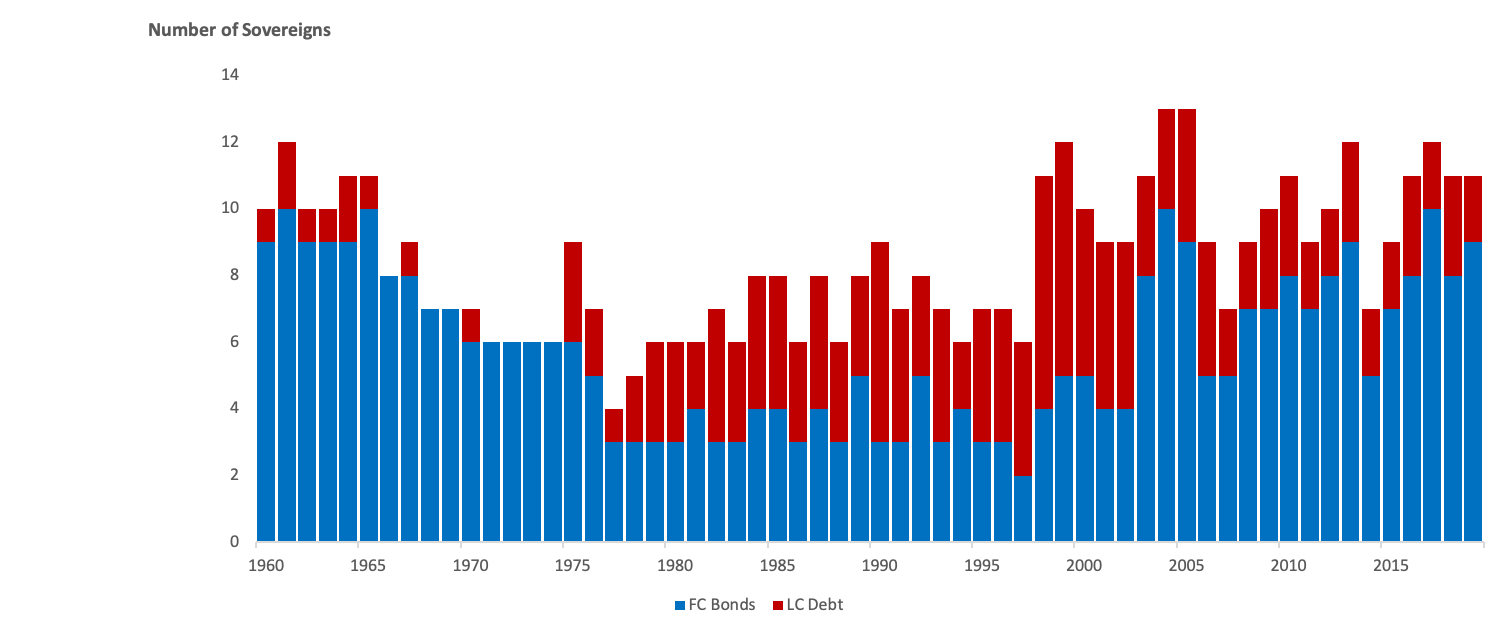
\includegraphics[trim={2.5cm 0cm 0.1cm 0cm},clip,width=0.9\textwidth,height=0.85\textheight]{../Figures/Slides/Defaults_FC_LC.png}
	\end{center}
	\begin{textblock*}{50mm}(17mm,85mm)
		\tiny Source: BoC-BoE Sovereign Default Database.
	\end{textblock*}
	\begin{textblock*}{5cm}(0.92\textwidth,1.07\textheight)
		\hyperlink{CreditRating}{\beamergotobutton{Credit Ratings}}
	\end{textblock*}
\end{frame}
\note{We generally assume that sovereigns rarely default on LC debt b/c in theory they can `print' their own currency.}
\note{This figure shows the number of sovereigns that have defaulted on foreign and LC debt since 1960.}
\note{The number of defaults on FC are in blue, while the number of defaults on LC are in red.}
\note{As you can see, defaults on LC debt do occur and are more common than is usually thought.}
\note{For instance, there have been more than 60 default episodes in LC since 1980, and more than 30 since 1996.} % , bonds denominated in LC
\note{One famous example of a LC default is Russia in 1998 but there are more recent examples like Barbados in 2018.}
\note{With the pandemic, last year several EMs saw deteriorations in their credit quality. For instance, credit rating agencies downgraded more than 35 sovereigns in 2020, mostly EMs, some of which unfortunately might end up defaulting in the future.} % (August 2020) % downgrades in LC bonds?

%\note{44 sovereigns with negative outlooks
%	EM public debt projected to be above 60\% of GDP (IMF)} % from 40\% of GDP after the GR
%\note{Analysis is informative for effective mitigation of undesired domestic impacts.}
%\note{Negative outlooks mean that more downgrades might be coming.}
%\note{Credit rating agencies have long recognized that possibility.}
%\note{Few EM have a credit rating of A and more than 30 have a rating below investment grade of BBB.}
%\note{Examples of overt defaults in LC debt: Barbados(2018), Jamaica (2013), Nicaragua (2008), Argentina (2001), Turkey (1999) (earthquake, retroactively taxed LC debt), Russia (1998) after high inflation, Brazil 1990.} %Mexico 1982. El Salvador 2017, Cyprus 2013?
%%It is true that LC defaults are less frequent than FC defaults but the number of domestic-law defaults has increased over time.
%
%\note{With the increase in foreign participation on LC bond markets in the 90s awareness of LC defaults increased.}
%\note{LC defaults have had limited visibility b/c:
%	- governments rarely acknowledge them. 
%	- bonds mostly held by domestic investors.}
%\note{Greater foreign participation in the 90s increased awareness of more recent default cases.} 
%\note{Foreign investor participation increased from 10\% in 2008 to 25\% in 2019.} % (W \& W, 2020)
%%\note{in 2011, G20 launched initiative to support LC bond markets in EM.}
%%LC default unlikely for countries with debt mainly in LC at long maturity.


\begin{frame}
	\frametitle{This Paper}
	How to \alert{decompose} the sovereign yields of emerging markets (EMs)?
	\begin{itemize}
		\item Accounting for credit risk
		\newline
	\end{itemize}
	
	How does U.S. monetary policy \alert{transmit} to EM sovereign yields? 
%	\begin{itemize}
%		\item Does it influence expectations of future policy rates? 
%		\item Does it affect the term premium?
%		\item Does it impact creditworthiness?
		\begin{itemize}
			\item Expectations of future policy rates? 
			\item Term premium?
			\item Creditworthiness?
		\end{itemize}
%	\end{itemize}
\end{frame}
\note{The main research question that I address in the paper is: How does US MP transmit to the sovereign bond yields of EMs?}
\note{To answer the question, I first propose a decomposition of the yields that explicitly takes into account the risk that EMs might default on their LC debt. I then use the decomposition to empirically quantify the effects of US MP surprises on each component.}

\note{There are three main findings that summarize the transmission channels of US MP to EM yields. But since they involve the components of the yields, let me show you a couple of figures to fix ideas.}


\begin{frame}
\frametitle{Traditional Yield Curve Decomposition}
\begin{center}
	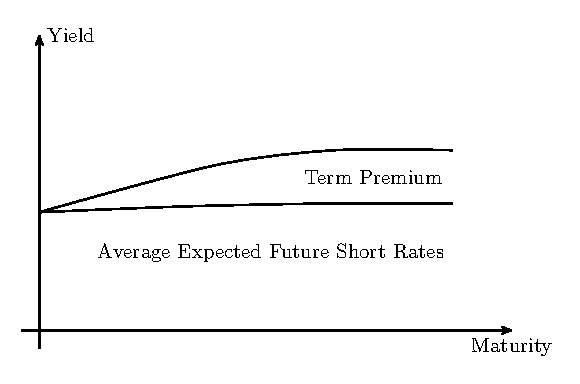
\includegraphics[trim={0cm 0cm 0cm 0cm},clip,width=0.85\textwidth,height=0.95\textheight]{../Figures/YC/ycdcmp_AE}
\end{center}
\end{frame}
\note{In this figure, you can see a stylized two-part decomposition of bond yields. The YC shows the relationship b/w bond yields at different maturities at a point in time. By assuming that the bonds are free of default risk, the yields can be decomposed into two parts: an average expected future short rate and a term premium.}
\note{A shortcoming of past work is to use this two-part decomposition for the yields of EMs b/c it ignores the fact that EMs do default.}


\begin{frame}
\frametitle{Proposed EM Yield Curve Decomposition}
\begin{center}
	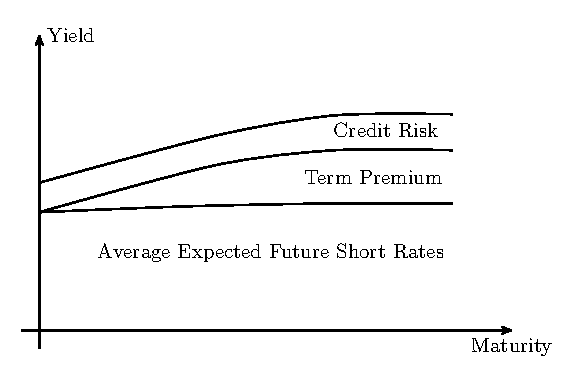
\includegraphics[trim={0cm 0cm 0cm 0cm},clip,width=0.85\textwidth,height=0.95\textheight]{../Figures/YC/ycdcmp_EM}
\end{center}
\end{frame}
\note{Instead of the traditional approach, I propose a three-part decomposition for the yields of EMs, which you can see schematically in this figure.}
\note{In addition to the usual two components, there is a third component that compensates investors for bearing credit risk, which is obtained as the difference between the usual nominal yield and a synthetic yield.}
\note{Later in the talk I will explain how synthetic yields are constructed but they essentially swap the US YC into a LC YC that can be considered free of credit risk, so the traditional two-part decomposition applies to them.}


\begin{frame}
	\frametitle{U.S. Monetary Policy Spillovers to EM Yields}
%	\begin{enumerate}
%		\item 
		1. Response of EM yields is \alert{economically significant}, yet \alert{delayed} %over days
		\begin{itemize}
			\item Response sometimes lasts longer in EM than in U.S. yields
			\newline
		\end{itemize}
		
		
%		\item 
		2. \alert{All three} components react to U.S. monetary policy % shocks <2->
		\begin{itemize}
			\item EM central banks expected to follow Fed's monetary stance
			\item EM term premia response is similar to U.S. term premium
			\item Fiscal implications in EMs of U.S. monetary policy
			\newline
		\end{itemize} 
	
%		\item 
		3. Unconventional policies \alert{limit} EM monetary autonomy along yield curve % yield <3>
		\begin{itemize}
			\item Global financial cycle more relevant at the long end
		\end{itemize}
%	\end{enumerate}
\end{frame}
\note{As I mentioned, three main findings summarize the transmission channels of US MP to EM yields.}

\note{First, the response of EM yields is economically significant and amplifies over the month following a MP surprise, which can be attributed to gradual adjustments in portfolio reallocations also known as slow-moving capital.} %  This is consistent with the evidence for advanced economies, since their yields display a similar sluggish response.
\note{I also find that, for certain types of surprises, the effects on EM yields last longer than on US yields.}

\note{Second, all 3 components of EM yields react, which means that surprises in US monetary policy lead investors to reevaluate their policy rate expectations and their perceptions of interest and credit risks in EMs.}
\note{For instance, I find that investors expect CBs in EMs to follow the monetary stance of the Federal Reserve rather than counteract its measaures. So if the Fed loosens or tightens financial conditions, EM CBs are expected to follow suit.}
\note{In addition, the UMP tools, namely FG and asset purchases, aimed at reducing the term premium in US yields also reduce the term premia in EM yields.}
\note{Moreover, the CRC part also reacts to US MP surprises. I highlight that the fiscal implications in EMs of MP in the US have so far not been discussed in the literature.}

\note{And third, since the 2007-2009 crisis the GFCy -which refers to the global comovement of risky asset prices- has a stronger impact on the LT yields than on the ST yields of EMs. Since Fed's decisions are important drivers of the GFCy, the unconventional policies implemented by the Fed after the GFC limit the influence central banks in EMs can exert over their domestic YCs.}


\begin{frame}[label=LitReview]
	\frametitle{Related Literature}
	
	\alert{Synthetic yields} and covered interest rate parity deviations
	\begin{itemize}
		\item {\scriptsize \cite{DuSchreger:2016JoF}; \cite*{DuImSchreger:2018JIE}; \cite*{DuTepperVerdelhan:2018}}
	\end{itemize}

	\alert{Sovereign default} in EM local currency bonds
	\begin{itemize}
		\item {\scriptsize \cite{ReinhartRogoff:2011}; \cite{DuSchreger:2016JoF}; \cite{ErceMallucci:2018}; \cite{OttonelloPerez:2019}}
	\end{itemize}
	
	\alert{Global financial cycle}
	\begin{itemize}
		\item {\scriptsize \cite{Rey:2013}; \cite{Turner:2014}; \cite{Obstfeld:2015}; \cite{Kalemli-Ozcan:2019}; \cite{KolasaWesolowski:2020}}
	\end{itemize}
	
	\alert{Spillovers} of U.S. monetary policy to EM yields
	\begin{itemize}
		\item {\scriptsize \cite{HausmanWongswan:2011}; \cite*{BowmanLondonoSapriza:2015}; \cite*{CurcuruKaminLiRodriguez:2018}; \cite*{Albaglietal:2019}; \cite*{ACDM:2019}}
	\end{itemize}
\end{frame}
\note{The paper relates to different branches in the literature.} % but in the interest of time, I will just point out two things.
\note{One branch uses synthetic yields to study deviations from covered interest rate parity.
	Another, documents the prevalence of sovereign defaults in LC.
	A branch describes different mechanisms through which US MP can transmit to the sovereign bond yields of EMs.
}
\note{Finally, several papers have studied the spillovers of US MP to bond yields. But there are two issues regarding the effects on EM yields.}
\note{First, the literature on term structures of EM yields has not examined credit risk systematically, it uses a two-part decomposition, which implicitly assumes that credit risk is zero and so EMs are treated as AEs.}
\note{Second, the analysis of spillovers using yield decompositions has mainly focused on AEs and, again, when EMs are included, they are treated as AEs.}


\section{Yield Curves}
\note{Is there any question? Let me start by explaining how to construct the YCs that will be decomposed later.}

\begin{frame}
\frametitle{Nominal Yield Curves}

	 Bloomberg par yield curves \(\rightarrow\) Zero-coupon yield curves (\(\yLCnom\))
	\begin{itemize}
		\item But \alert{credit risk} in \(\yLCnom\) %LC nominal yields of EM
	\end{itemize}
	
	\textbf{Approach}: \alert{Synthetic} LC yields (\(\yLCsynt\)) as \textit{free of credit risk}
	\begin{itemize}
		\item Swap U.S. Treasury yields into LC yields using currency derivatives
	\end{itemize}
	
	\textbf{Assumption}: Frictionless financial markets \citep{DuSchreger:2016JoF}
	\begin{itemize}
		\item Arbitrageurs have access to U.S. and LC bonds
		\item Derivatives have no counterparty risk
		\item U.S. yields are free of default risk
	\end{itemize}
	
%	Why not CDS (credit default swaps)?
\end{frame}
\note{The nominal YCs are ZC YCs obtained from the par YCs reported by Bloomberg but, as I mentioned in the introduction, it is not appropriate to use the traditional decomposition on these yields b/c it ignores the credit risk embedded in them.}
\note{To explicitly account for credit risk, I use synthetic yields, which essentially swap the US YC into a LC YC that can be considered free of credit risk. In this sense, synthetic yields represent the borrowing costs of a hypothetical bond issuer in LC w/ no credit risk.}
\note{Under this approach, the US YC serves as a benchmark for all EMs. The approach assumes frictionless financial markets, that is}
\note{Global investors have unrestricted access to US and LC bonds. The derivatives used in the construction of the synthetic yields have no counterparty risk and US yields are free of default risk.}
\note{There are circumstances in which these assumptions migh not hold exactly. However, \cite{DuSchreger:2016JoF} show that these assumptions are a \alert{useful benchmark} to study credit risk in EM yields.} % In the analysis, I rely on the work of 

\note{An alternative approach to synthetic yields is to use CDS. I do not use them mainly because the definition of default is not always clear. Plus, ISDA does not include defaults on LC bonds governed under domestic law as triggers of CDS payouts.}
%\note{CDS do not adequately characterize LC credit risk.}
%\note{Broad perspective on credit risk, i.e. not receiving promised payments: EMs can change the law + Suspension of currency convertibility + Capital controls + Actual default.}
%\note{BFV curves are par yield curves provided by Bloomberg on a daily basis for different maturities. To obtain the implied zero-coupon curves, the yields are converted into discount factors, which are then used to estimate the parameters of the Nelson-Siegel-Svensson model.}
%\note{CDS is a financial derivative that enable investors to swap credit risk.}


\begin{frame}[label=Synthetic]
\frametitle{Synthetic Yield Curves}
%\vspace{-1cm}
\begin{equation*} \label{eq:uLCsynt}
	\eqyLCsynt
\end{equation*}
%\vspace{-0.5cm}

	\(\yLCsynt\): \(\tnr\)-period zero-coupon \textit{synthetic} yield in LC at time \(\idxt\) % (\(\yLCnom\) not needed)
	
	\(\yUS\): \(\tnr\)-period zero-coupon U.S. yield at time \(\idxt\) % (in USD)
	
	\(\fwdprm\): \(\tnr\)-period foreign exchange \alert{forward premium} from USD to LC at time \(\idxt\)
%	\begin{itemize}
%		\item Currency forwards (\(< 1\) year) and cross-currency swaps (\(\geq 1\) year)
%	\end{itemize}
	
	\begin{itemize}
		\item \alert{\(< 1\) Year}: Currency forwards
%		\[(forward_{t,\tnr} - spot_{t})/\tnr\]
		\item \alert{\(\geq 1\) Year}: Cross-currency swaps %Fixed-for-fixed 
		%	\iftoggle{long}{\pause}{}
		\begin{itemize}
			\item Interest rate swaps
			\item Cross-currency basis swaps
		\end{itemize}
	\end{itemize}
%	\begin{textblock*}{3cm}(.92\textwidth,0.74\textheight)
%		\hyperlink{FwdPrm}{\beamergotobutton{FP}}
%	\end{textblock*}
\end{frame}
\note{Synthetic yields are constructed by adding a FX forward premium to US yields.}
\note{This FP compensates investors for the expected depreciation of the LC.}
\note{For maturities of less than 1Y, the FP is calculated as the annualized difference b/w the forward and the spot exchange rates.}
\note{For maturities greater than or equal to 1Y, the FP is calculated using cross-currency swaps b/c outright forwards are less liquid.}
\note{When XCS are not directly traded in the market, they can be constructed using CCS and IRS based on the following sequence of steps.}
\note{Today I can lock in a risk-free investment in LC by exchanging LC for US dollars, investing those dollars in Tresuaries and entering into a forward contract agreeing to sell dollars for LC in the future.}
\note{Once the dollar payment from the investment in Treasuries is received, those dollars are exchanged back into LC at the agreed forward exchange rate.}
\note{All the derivative instruments involved are liquid and collateralized so the bilateral counterparty risk is small.}
\note{Notice that the nominal YC is not needed in the construction of the synthetic YC.}


\begin{frame}[label=DevCIP]
\frametitle{Deviations from CIP (Covered Interest Parity)}
%\vspace{-0.5cm}
\[\eqCIPdevDS\]

\vspace{0.2cm}
	Measures:
	\begin{itemize}
		\item \alert{Convenience yield} for AEs \citep*{DuImSchreger:2018JIE}
%		\item[] {\small \cite*{DuImSchreger:2018JIE}} 
		\item \alert{Sovereign credit risk} for EMs \citep{DuSchreger:2016JoF}
%		\item[] {\small \cite{DuSchreger:2016JoF}} 
		\item \alert{Financial frictions} for banks \citep*{DuTepperVerdelhan:2018} \newline
%		\item[] {\small \cite*{DuTepperVerdelhan:2018}}
	\end{itemize}

	\textbf{Here}: Emphasis also on \(\yLCsynt\)
\end{frame}
\note{Synthetic yields can be constructed, as I just explained, for both AEs and EMs.}
\note{The spread b/w the nominal and the synthetic yields measures deviations from CIP in government yields.}
\note{But the interpreation of the spread depends on the context.}
\note{For AEs, Du, Im and Schreger document that the spread measures the difference in the convenience yield of investing in US Treasuries relative to the convenience yield of investing in the bonds of other AEs.}
\note{For EMs, Du and Schreger document that the spread captures the compensation for credit risk. In particular, they show that the spread for EMs is highly correlated with their CDS.}
\note{While previous literature focuses on the spread, I emphasize the importance of the synthetic yields themselves given that they can be considered as free of credit risk and so the traditional two-part decomposition can be applied to them.}
%\note{Correlation b/w CIP dev and CDS is high for EMs but not for AEs.}


\begin{frame}[label=YldData]
\frametitle{Yield Data}
	\alert{15 EMs}:
	\begin{itemize}
%		\item[] {\scriptsize BRL, COP, HUF, IDR, ILS, KRW, MYR, MXN, PEN, PHP, PLN, RUB, THB, TRY, ZAR}
		\item {\small Brazil, Colombia, Hungary, Indonesia, Israel, Korea, Malaysia, Mexico, Peru, Philippines, Poland, Russia, Thailand, Turkey, South Africa}
	\end{itemize}
	%	\begin{itemize}
	%		\item \scriptsize \alert{10 AEs}: AUD, CAD, CHF, DKK, EUR, GBP, JPY, NOK, NZD, SEK
	%	\end{itemize}
%	\iftoggle{struct}{\item<2->}{\item} 
	
	\alert{Daily} data: January 2000 to January 2019
%	\iftoggle{struct}{\item<3->}{\item}
	
	\alert{Maturities}: 0.25, 0.5, 1, 2, \ldots, 10 years
%	\iftoggle{struct}{\item<4->}{\item}
	
	\alert{Synthetic} yields:
	\begin{itemize}
%		\iftoggle{struct}{\item<5->}{\item}
		\item $\yUS$: CRSP risk-free rates; \citet*{GSW:2007}
%		\vspace{-0.1cm}
%		\iftoggle{struct}{\item<6->}{\item}
		\item $\fwdprm$: Bloomberg; Datastream
	\end{itemize}

\begin{textblock*}{3cm}(.9\textwidth,1.052\textheight)
	\hyperlink{YldStats}{\beamergotobutton{Summary Statistics}}
\end{textblock*}
\end{frame}
\note{I construct nominal and synthetic yields for the 15 EMs originally studied by Du and Schreger at the daily frequency going back to 2000 up to 2019.}
\note{However, starting dates vary by country. Longer series are of course desirable to pin down the term premium since it is an unobserved variable. But there are at least 10 years of data for most countries in the sample, which is a reasonable sample size for the estimation of the models that I will explain in a moment.}
\note{The maturities considered in the analysis are 3M, 6M and from 1 to 10Y.}
\note{The construction of the synthetic yields uses the dataset built by GSW, which captures the US YC reasonably well for maturities greater than or equal to 1Y.}
\note{For the yields at the 3M and 6M maturities, I use data from CRSP b/c it is more robust at the short end of the YC.}
\note{Finally, the data for the forwards and swaps needed to compute the FP comes from BLP and DTS.}
%\note{Bonds\(>10Y\) have less history and are less liquid, including the swaps used to construct the synthetic YC.}

%\note{Results are compared against those obtained for 10 AEs.}
%\note{Reasons for use monthly: VAR is a good approximation for monthly, adequate frequency if want to use macro data.}


\section{Affine Term Structure Model}
\note{Let me now describe the model used for the decomposition of the yields.}

\begin{frame}[label=ATSMsummary]
\frametitle{Model Overview}
	
	Standard discrete-time nominal affine term structure model
	\begin{itemize}
		\item Assumes default-free bonds \(\rightarrow\) \alert{Synthetic} yields (\(\yLCsynt\)) for EMs
		\item \alert{Augmented} with survey forecasts
	\end{itemize}
	
	Intuition:
	\begin{itemize}
		\item Yields driven by pricing factors \(\Xvars\)
		\item Dynamics of pricing factors (\(\Pmeasure\) and \(\Qmeasure\) measures)
		\item No-arbitrage restrictions ensure consistency % in cross section / time series of yields
%		\item Yields are affine functions of the pricing factors
	\end{itemize}
	
	\begin{textblock*}{3cm}(0.08\textwidth,1.05\textheight)
	\hyperlink{AssetPricing}{\beamergotobutton{Asset Pricing}}
	\end{textblock*}
	\begin{textblock*}{3cm}(0.23\textwidth,1.05\textheight)
		\hyperlink{SDF}{\beamergotobutton{SDF}}
	\end{textblock*}
	\begin{textblock*}{3cm}(0.32\textwidth,1.05\textheight)
		\hyperlink{BondPrices}{\beamergotobutton{Bond Prices}}
	\end{textblock*}
	\begin{textblock*}{3cm}(0.46\textwidth,1.05\textheight)
		\hyperlink{SvyAugModel}{\beamergotobutton{Augmented Version}}
	\end{textblock*}
\end{frame}
\note{I use a discrete-time nominal ATSM, which is a standard tool to estimate the dynamics of risk-free *nominal* YCs. The traditional decomposition relies on this risk-free assumption and that is why it makes sense for the bonds issued by AEs.}
\note{In the case of EMs, I use the model to capture the dynamics of the *synthetic* yields b/c they are better aligned with the risk-free assumption in contrast to the nominal yields.}
\note{I augment the model with survey forecasts of future ST interest rates to obtain robust decompositions as I will explain in a moment.}
\note{In the interest of time, I will not go into the details of the model but the intuition behind it is as follows.}
\note{According to the model, bond yields are driven by a set of pricing factors whose actual dynamics are represented with simple vector autoregressions.}
\note{Restrictions are then imposed to reflect the no-arbitrage condition across maturities, giving rise to alternative, risk-adjusted dynamics for yields. The actual and the risk-adjusted dynamics are also known as the P and the Q measures.}
\note{The difference between the P and Q dynamics reflect market participants' risk preferences. By exploiting these two dynamics, yields can be decomposed into expectations of future interest rates and term premia.}
%\note{The coefficients are functions of the maturity of the bond and the coefficients that determine the stochastic processes that drive the state variables.}


\begin{frame}[label=Components]
\frametitle{EM Yield Decomposition}
\vspace{-0.35cm}
\[\yLCnom \; \; = \; \; \yZeroQ \; + \; \CIPdev \; \; = \; \; \yZeroP \; + \; \termprm \; + \; \CIPdev \]

\vspace{0.8cm}
\begin{tabular}{ l l }
	\(\eqyZeroQ\) \(:\) & Fitted \alert{synthetic} yields \\ [15pt]
	
	\(\eqyZeroP\) \(\, :\) & Average expected future short rates \\  [15pt]
	
	\(\eqTP\) \(\; :\) & Term premium \\ [15pt]
	
	\(\CIPdev = \yLCnom - \yZeroQ\) \(\, :\) & Credit risk compensation
\end{tabular}
\end{frame}
\note{Here you can see how the nominal yields of EMs can be decomposed into three parts.}
\note{The nominal yields are equal to the risk-free synthetic yields plus a compensation for credit risk. Since synthetic yields are seen as free of credit risk, they can be decomposed into an average expected short rate and a term premium.}
\note{The CRC part has been ignored in previous work by assuming that the nominal yields are free of credit risk.}
\note{Therefore, the TP that I propose is *clean* in the sense that it is not contaminated with credit risk as would be the case with traditional approach. In other words, using the traditional approach for EM yields would generate a term premium contaminated with credit risk.}

\note{The fitted synthetic yields are given as affine functions of the pricing factors using parameters under the Q measure. The average expected future short rates are also affine functions of the pricing factors but under the P measure. The difference b/w the two gives an estimate for the term premium. Finally, the spread b/w the nominal and the fitted synthetic yields is the CRC.}
\note{Since the model fits the synthetic yields reasonably well, as you will see in a moment, this spread is largely similar to the one reported by Du and Schreger, and which they referred to as the LC credit spread.}
\note{Of course, the spread might not be a perfect measure of credit risk but it is *definitely* better than ignoring it.}


\begin{frame}
\frametitle{Weak Identification}

Yields \alert{accurately} identify \(\Qmeasure\) parameters, yet \(\Pmeasure\) ones are \alert{poorly} identified % , yet parameters % \{\(\XmuQ, \XPhiQ\)\} % \{\(\XmuP, \XPhiP\)\}

\begin{itemize}
	\item Bond yields are persistent
	\item Unstable yield decompositions
\end{itemize}

\textbf{Solutions}: Survey data, parameter restrictions, bias-corrected estimators

Surveys provide \alert{robust} decompositions of AE yields \citep{Guimaraes:2014}
\begin{itemize}
	\item Surveys anchor the long run mean of interest rates.
	\item Important for EM yields given small sample sizes
\end{itemize}
\end{frame}
\note{The estimation of the parameters in the model only requires data on yields, which accurately identifies the parameters under the Q measure.}
\note{However, the parameters under the P measure are poorly identified since bond yields are persistent and the term premium is an unobserved variable, which can result in unstable yield decompositions.}
\note{That is why it is desirable to have long series for the estimation.} % This is a problem given that the TP is an unobserved variable. 
\note{Different solutions have been proposed in the literature like complementing yield data with surveys on interest rate forecasts (especially long-term forecasts), imposing restrictions on the parameters and using bias-corrected estimators.}
\note{Guimaraes compares those solutions and concludes that surveys provide robust decompositions for the YCs of the US and the UK.}
\note{In particular, surveys are useful becase help the model anchoring the long run mean of interest rates.}
\note{In the case of EM, it is especially important to use surveys given the relatively small sample sizes compared to those for AEs.}

%Most variability attributed to fluctuations in term premium
% Overestimates stability of expected path of short rate
%\note{Although the estimation of the parameters in the model only requires data on yields, it can result in unstable yield decompositions because bond yields are persistent and the TP is an unobserved variable.}
%\note{It has been shown that surveys provide robust decompositions for the YCs of AEs; they help anchoring the long run mean of interest rates.}

%\note{Overestimates stability of expected path of short rate}
%\note{Surveys are an effective solution to obtain robust decompositions of the yield curve \citep{Guimaraes:2014} 


\begin{frame}[label=SCBP]
\frametitle{Survey Data}

No data on long-term forecasts for EM short rates

Implied forecast for EM short rates from existing data %on long-term forecasts

\begin{equation*} \label{eq:uRrt}
	\eqrrt
\end{equation*}

\begin{itemize}
\item \alert{EM inflation} forecasts: 5 years ahead and long-term
\begin{itemize}
	\item From Consensus Economics (CE), available twice a year
\end{itemize}

\item Implied long-term expectations of \alert{U.S real interest rate} using
\begin{itemize}
\item T-bill rate, CPI inflation from Survey of Professional Forecasters (SPF)
%\item Compared against TIPS yields
\end{itemize}
\end{itemize}

\begin{textblock*}{3cm}(.9\textwidth,1.05\textheight)
	\hyperlink{YldCBP}{\beamergotobutton{Implied Forecasts}}
\end{textblock*}
\end{frame}
\note{Unfortunately, there is no data on LT forecasts for the short rates of EMs.}
\note{Consensus Economics, for instance, provides long-horizon forecasts for consumer inflation and real GDP growth but not for ST rates.}
\note{So I infer the forecasts from existing data using the Fisher equation and treating EMs as SOEs, which implies that the global real interest rate is determined abroad.}
\note{This approach requires forecasts for inflation in each EM and for the global real interest rate.}
\note{Inflation forecasts come from CE and are available twice a year.}
\note{The U.S. real interest rate serves as a proxy for the global real interest rate and is derived using forecasts for the T-bill rate and CPI inflation from the SPF.}
\note{This calculation is done using 5Y- and 10Y-ahead forecasts.} % and b/w 5Y and 10Y ahead forecasts
%\note{I compare them also against the real yields from TIPS and against an alternative approach using Taylor-rule type regressions, which also use forecasts for real GDP. The results are also comparable.}


\begin{frame}
\frametitle{Model Estimation}

%	\item Use \cite*{JSZ:2011} normalization of the model %: \(\Pmeasure \perp \Qmeasure\) % likelihood functions
Estimate parameters by ML with \alert{monthly} data on yields
\begin{itemize}
\item \cite*{JSZ:2011} normalization
\end{itemize}
%	\item Estimate \(\Pmeasure\) parameters by OLS
%	\item Estimate \(\Qmeasure\) parameters by MLE

Estimate survey-augmented model by Kalman filter (missing data)
\begin{itemize}
\item Surveys as \alert{`noisy'} expectations measures \citep{KimOrphanides:2012}
\end{itemize}

Standard errors by delta method

Estimate pricing factors at \alert{daily} frequency

\end{frame}
\note{I estimate the model using end-of-month data and a two-step approach.}
\note{First, the model is estimated by ML using only data on yields and following the normalization proposed by JSZ, which essentially separates the likelihood function of the model into likelihoods for the P and the Q measures.}
\note{The estimated parameters obtained in this way are used as initial values in the second step, in which yields are complemented with survey data.}
\note{Since surveys are available twice a year, they are treated as mising values in the months in which no surveys are released.}
\note{The survey-augmented model is thus estimated by the KF b/c it can easily handle missing data.}
\note{Although surveys contain useful information that helps anchoring the model to reality in each country, they are not a panacea, so they are treated as `noisy' measures of expectations by using a conservative value for their standard deviation following Kim and Orphanides.}
\note{Finally, I use the parameters obtained with monthly data to estimate the pricing factors at the daily frequency. This allows me to perform daily decompositions of the yields, which are needed to analyze the persistence of the MP decisions in the US.}
%\note{At the daily frequency there is noise in yield data that can undermine the estimation.}


\section{EM Yield Decomposition}
\note{Now I will show you how well the model fits the data and how the decomposition looks like.}

\begin{frame}[label=ModelFit]
%	\frametitle{Model Fit}
\vspace{0.2cm}
\begin{center}							% center the figure inside the minipage
\includegraphics[trim={0cm 0cm 0cm 0cm},clip,height=0.95\textheight,width=\linewidth]{../Figures/Estimation/s_ylds_bsl_yQ.eps} \\
\end{center}
\begin{textblock*}{15cm}(2.5mm,3mm)
	\textbf{10Y}
\end{textblock*}
\end{frame}
\note{This figure illustrates the fit of the model for the 10Y synthetic yields of all the countries in the sample. The actual yields are in blue and the fitted yields are in orange.}
\note{As you can see, the model fits the data reasonably well.}


\begin{frame}[label=YldDcmp2]
%	\frametitle{Decomposition of EM Nominal Yields}
\begin{center}							% center the figure inside the minipage
%\includegraphics[trim={0cm 0cm 0cm 0cm},clip,height=0.95\textheight,width=\linewidth]{../Figures/Estimation/ny_dcmp.eps} \\
\includegraphics[trim={0cm 0cm 0cm 0cm},clip,height=0.95\textheight,width=\linewidth]{../Figures/Estimation/HUF_MXN_dcmp.eps} \\
\end{center}
\begin{textblock*}{15cm}(2.5mm,3mm)
	\textbf{10Y}
\end{textblock*}
%\begin{textblock*}{3cm}(.23\textwidth,1.08\textheight)
%	\hyperlink{yPscbp}{\beamergotobutton{Expected Short Rates}}
%\end{textblock*}
\begin{textblock*}{3cm}(.23\textwidth,1.08\textheight)
	\hyperlink{YldDcmp10}{\beamerreturnbutton{Decomposition All}}
\end{textblock*}
\begin{textblock*}{3cm}(.51\textwidth,1.08\textheight)
\hyperlink{tpCI}{\beamergotobutton{Term Premia}}
\end{textblock*}
\begin{textblock*}{5cm}(.725\textwidth,1.08\textheight)
\hyperlink{crcCI}{\beamergotobutton{Credit Risk Compensation}}
\end{textblock*}
\end{frame}
\note{In this figure you can see how the decomposition looks like over time for the 10Y nominal yields for HUF and MXN, which are two of the countries in the sample.}
\note{The solid blue line is the AESR. The dash-dotted orange line is the TP. And the dashed yellow line is the CRC.}
\note{On average, the ESR explains most of the variability in yields. However, the dynamics of the TP and the CRC are also important drivers of EM bond yields, yet the TP plays a relatively bigger role than the CRC, in general.}
\note{It is encouraging that the decomposition captures local conditions in each country.}
\note{For instance, the CRC for HUF increased after 2010, when the current populist government came into power.}
\note{In the case of MX, the CB started a tightening cycle following the 2016 US presidential election, in response to a depreciation of the currency. That move is reflected in an increase in ESR.}
\note{To assess the decomposition more generally, I study the components by themsevles but focusing on the ESR and the term premium b/c D-S already study the CRC in detail; as I mentioned before, they show that it is highly correlated with CDS.}

%\note{Since 2011 there has been strong demand for LC bonds in Asia, which partly explains TP < 0 seen in Asian countries.}
%\note{TP decline due to: international investors, US UMP.}

%\note{USTP increased around the onset of the Great Recession (September 2008), the taper tantrum (June 2013), and the 2016 U.S. presidential election (November 2016), while it declined after the first unexpected announcement of the QE program by the Fed (March 2009).}
%\note{Common explanations for the decline in the USTP include an increased demand of U.S. assets by global investors and the effects of the UMP of the Fed.}
%\note{Explanation for change in sign (Campbell, Sunderam \& Viceira (2016)): TP < 0 is explained by the flip in the sign of the correlation between stocks and bonds -bonds hedge stocks-.}
%\note{Events: GR, TT, US election, 2009 QE1.}


\begin{frame}[label=yPscbp]
%	\frametitle{Components: Expected Future Short Rate}
\vspace{0.1cm}
\begin{center}							% center the figure inside the minipage
	\includegraphics[trim={0cm 0cm 0cm 0cm},clip,height=0.95\textheight,width=\linewidth]{../Figures/Estimation/bsl_yP_scbp.eps} \\
\end{center}
\begin{textblock*}{15cm}(2.5mm,3mm)
	\textbf{10Y}
\end{textblock*}
%\begin{textblock*}{5cm}(0.97\textwidth,1.05\textheight)
%	\hyperlink{YldDcmp10}{\beamerreturnbutton{Decomposition}}
%\end{textblock*}
\end{frame}
\note{This figure compares the 10Y ESR implied by the model in blue and the 10Y forecast for the short rate in orange. You can see that the model implied value tracks the forecast reasonably.}


\begin{frame}[label=tpUCSV]
\frametitle{Term Premium and Inflation Uncertainty}

\alert{Term premia} in AEs compensates for \alert{inflation uncertainty} \citep{Wright:2011} \newline
%In advanced economies related to inflation uncertainty \citep{Wright:2011} % in advanced economies

\alert{Inflation} higher and \alert{more volatile in EMs} than in AEs \citep{HaKoseOhnsorge:2019}
\newline

\textbf{Question}: Is inflation uncertainty relevant for EM term premia?

\vspace{-0.5cm}
\begin{equation*} \label{eq:uPanelUCSV}
	\eqpanelUCSV ,
\end{equation*}

\begin{itemize}
	\item \(\sigma^{\pi}_{\idxspnl}\) of permanent component in UCSV model \citep{StockWatson:2007}
	\item \(GDP_{\idxspnl}\) controls for the business cycle
\end{itemize}
\end{frame}
\note{To assess the validity of the estimated TP, two findings in the literature are worth highlighting. The first one is that the TP compensates investors for bearing inflation uncertainty in AEs and the second is that inflation is higher and more volatile in EMs than in AEs.}
\note{Therefore, it is reasonable to assume that the relationship between the term premium and inflation uncertainty is particularly relevant in EMs.}
\note{To test this hypothesis, I regress the term premium on a measure of inflation uncertainty controlling for the business cycle, which is proxied by the growth rate in real GDP.}
\note{Following Wright, the measure of inflation uncertainty is the standard deviation of the permanent component of inflation based on the unobserved components stochastic volatility (UCSV) model of Stock and Watson.}


\begin{frame}
\frametitle{EM Term Premia and Inflation Uncertainty}
%	\setbeamercolor{background canvas}{bg=}
%	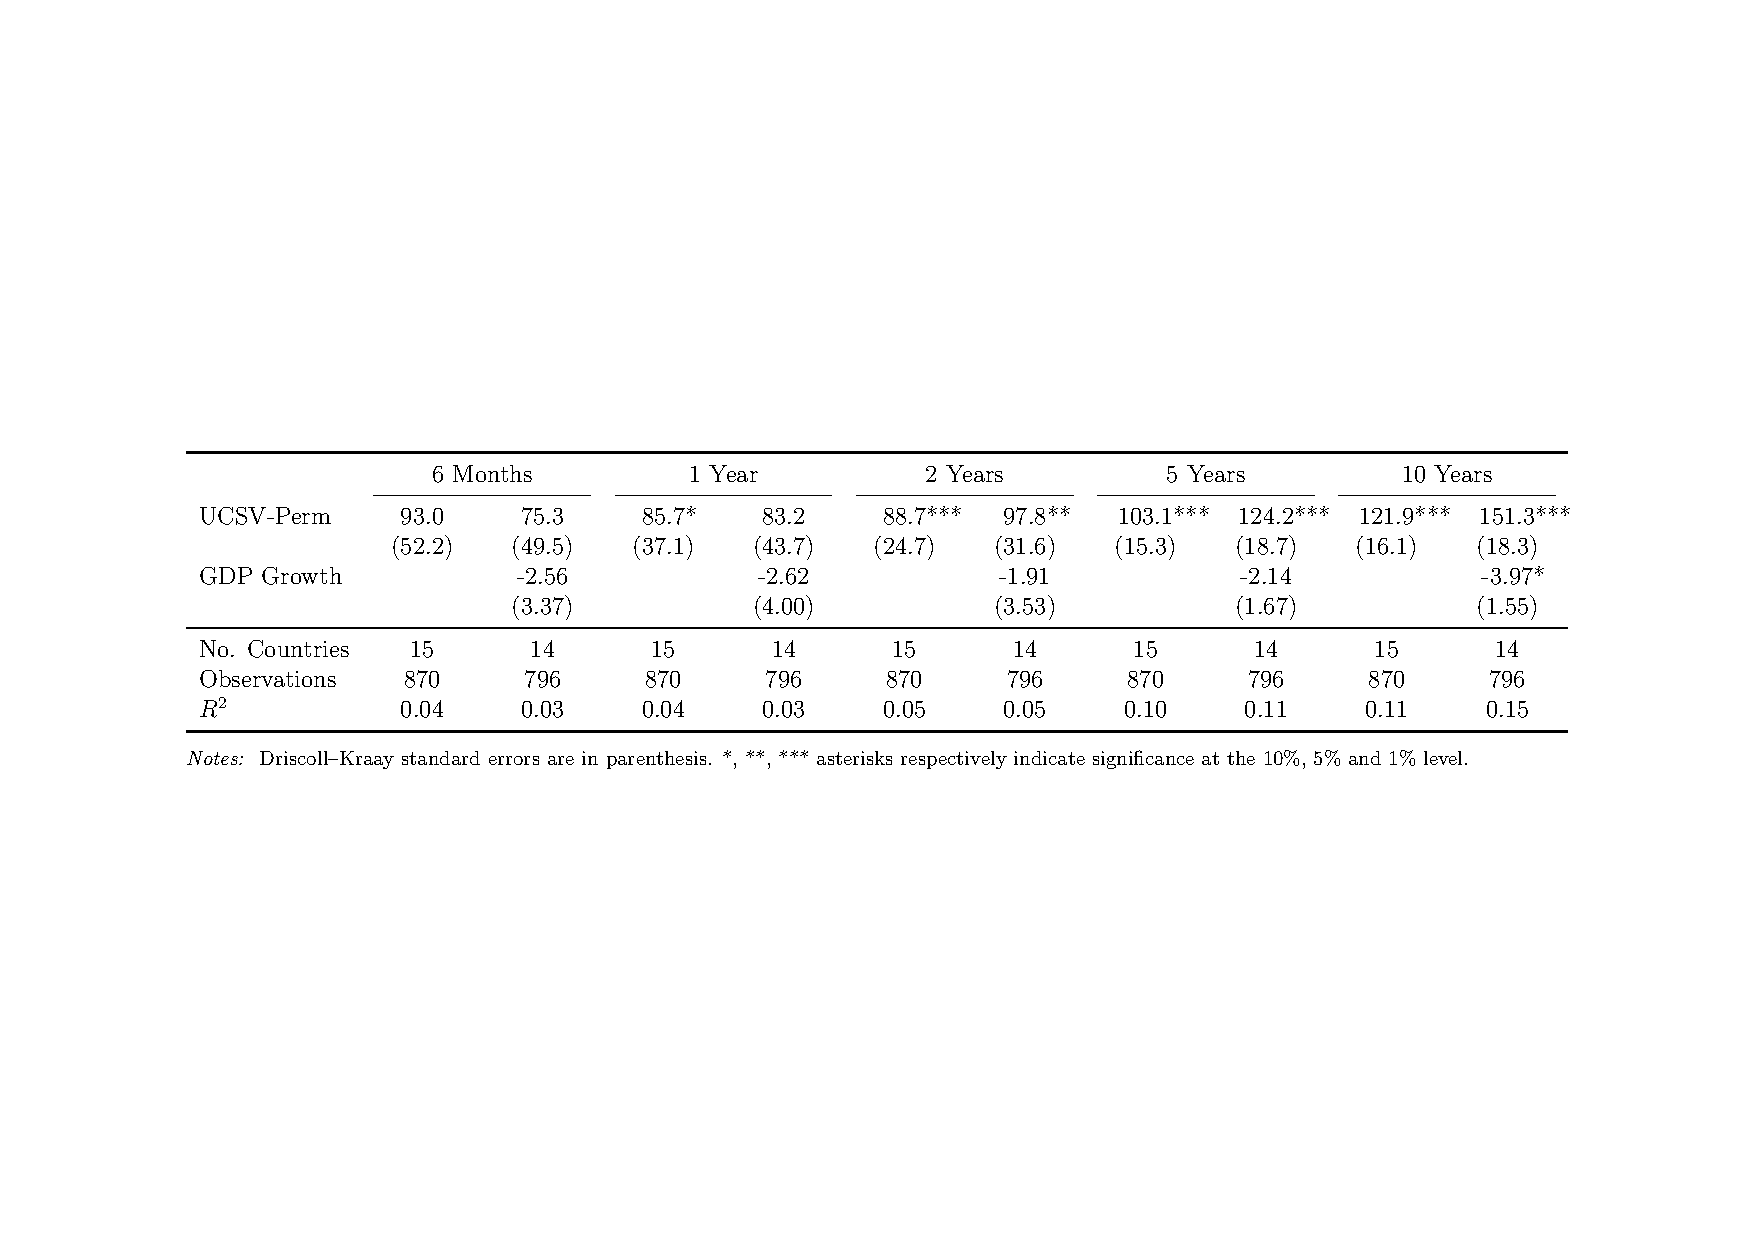
\includepdf[pages={1}]{../Tables/tpucsv.pdf}
\vspace{-0.8cm}
\begin{figure}[!htbp]
\begin{center} % trim removes: left, down, right, top
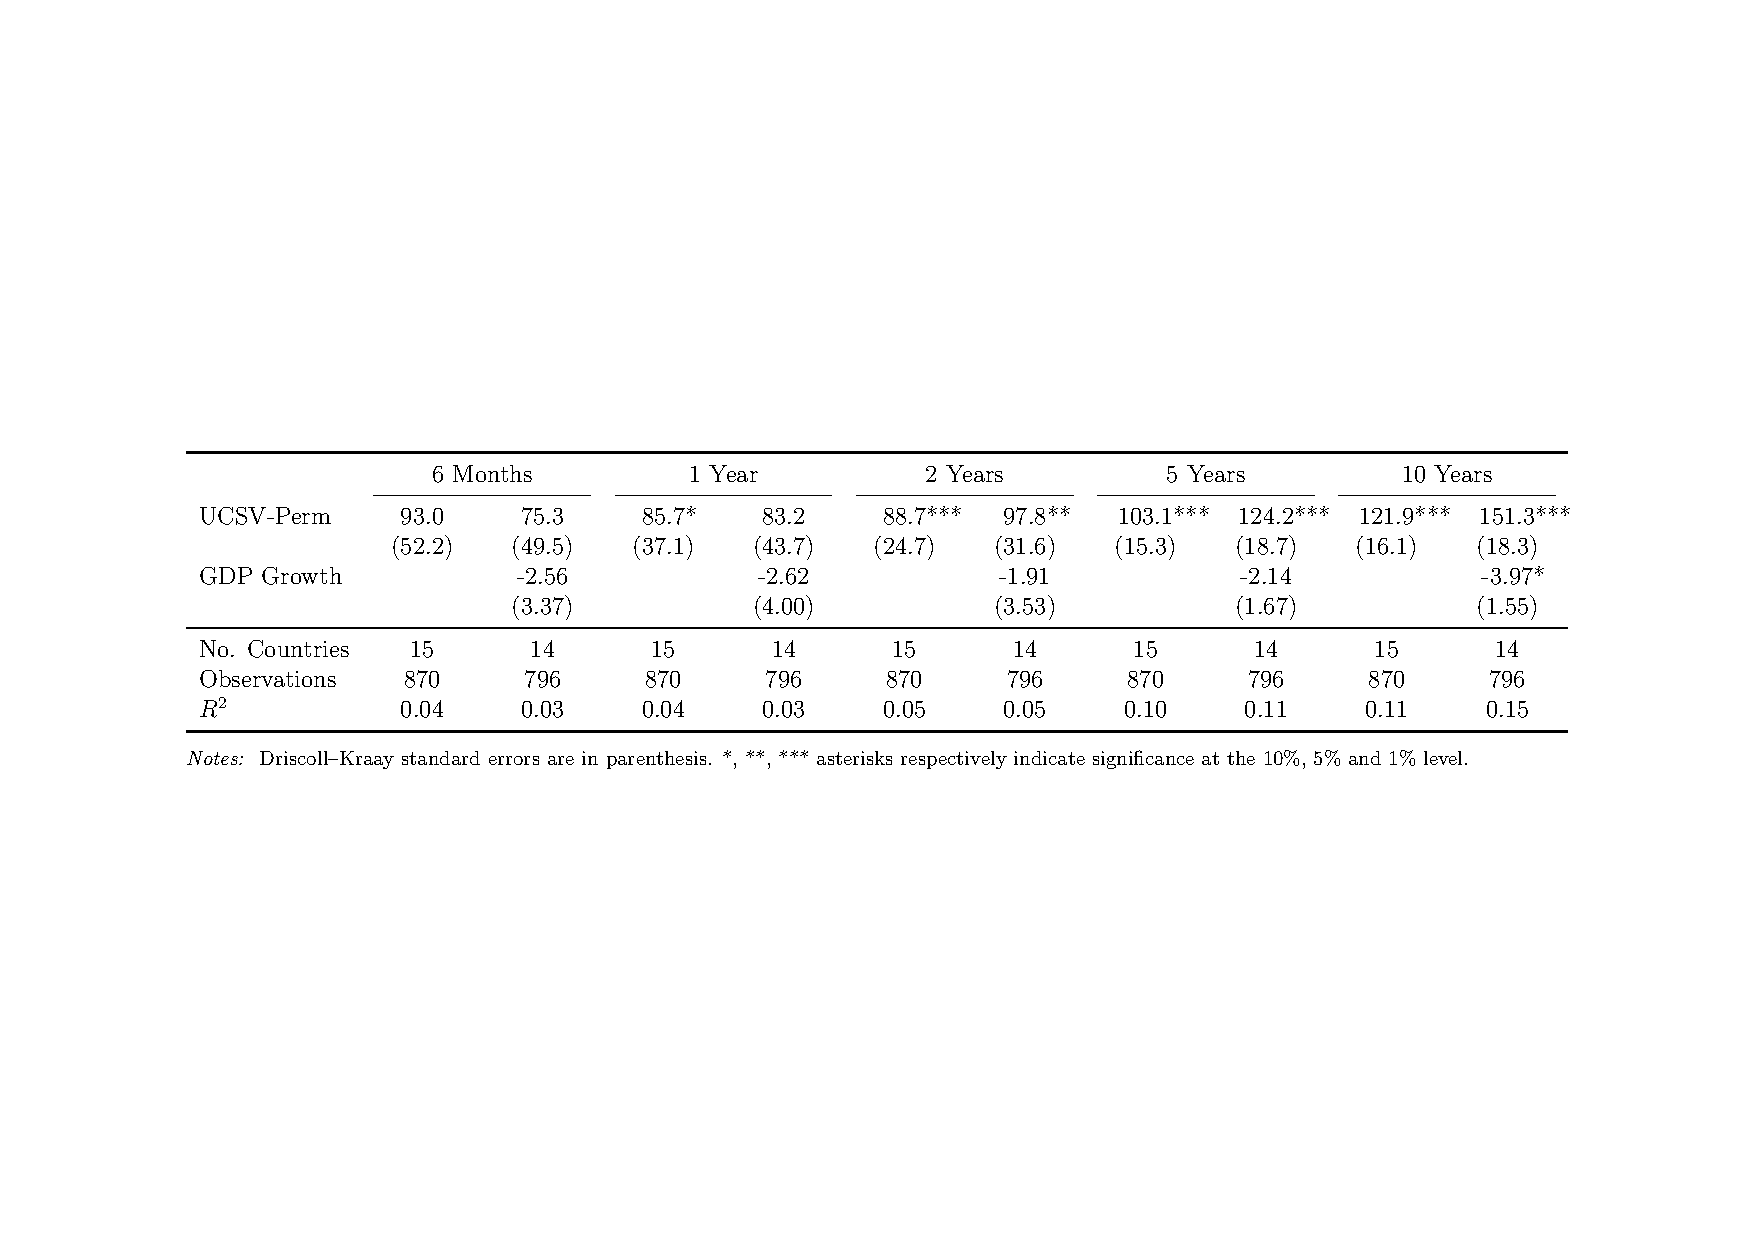
\includegraphics[trim={2.5cm 6cm 2.5cm 6cm},clip, width=1\textwidth,height=0.95\textheight]{../Tables/tpucsv.pdf}
\par\end{center}
\end{figure}
\end{frame}
\note{In this table, you can see that the standard deviation of the permanent component of inflation is indeed positively associated with the term premia in EMs.}
\note{Notice that the result increases with maturity and that it becomes stronger after controlling for the business cycle.}
\note{Even though the specification might be subject to econometric problems like persistent variables, the results are aligned with the view that term premia in EMs compensate investors for bearing inflation uncertainty.}


\section{U.S. Monetary Policy Spillovers}
\note{With the decomposition at hand for the 15 EMs, I now use it to address the main question about the transmission channels of US MP to EM yields.}

\begin{frame}
\frametitle{The Yield Curve Channel}
U.S. monetary policy key driver of the global financial cycle \citep{Rey:2013}

%Yield curve channel
%\begin{itemize}
	\alert{Long-term yields} more influenced by global forces
	\begin{itemize}
		\item EM \alert{monetary autonomy} declines along yield curve \citep{Obstfeld:2015}
	\end{itemize}

	U.S. \alert{unconventional} monetary policies affect EM yields
	\begin{itemize}
		\item Long-term via the term premium \citep{Turner:2014}
		\item Short-term via expected short rate \citep{Kalemli-Ozcan:2019}
	\end{itemize}
%\end{itemize}
\end{frame}
\note{The literature describes different mechanisms that I referred to as the YC channel, which can be explained as follows.}
\note{The GFCy, which refers to fluctuations in financial activity on a global scale, is mainly driven by developments in the US.} % One the three main findings that I mentioned in the introduction is related to t
\note{At the same time, a widely held view is that LT yields are more influced by global forces than ST ones. In the case of EMs, these global forces would limit the monetary autonomy of their CBs along their YCs.}
\note{In particular, the UMPs implemented by the Fed aimed at reducing the term premium in US yields can reduce EM yields by decreasing the TP in LT yields and the expected component in ST yields; this last effect is what K-O refers to as risk spillovers.}

%\note{We usually think that CBs exert control over a ST interest rate and financial markets transmit the monetary stance to LT interest rates.}


\begin{frame}
\frametitle{Implications of Yield Curve Channel}

Long-term EM yields \alert{comove more} than short-term ones

\alert{Direct} relationship that varies by maturity
\begin{itemize}
\item U.S. term premium \(\rightarrow\) EM term premium
\item U.S. expected future short rates \(\rightarrow\) EM expected future short rates
\end{itemize}

\alert{Cross} relationships at the \textit{short end}
\begin{itemize}
\item \textbf{Risk spillovers}: U.S. term premium \(\rightarrow\) EM expected future short rates
\end{itemize}
\end{frame}
\note{If there is a YC channel, we should observe that LT yields are more correlated than ST ones.}
\note{Also, there should be a direct relationship that varies by maturity b/w the term premia in the US and in EMs, and b/w ESRs in the US and in EMs.}
\note{If there are risk spillovers, we should observe that the US TP influences the ESR particularly at the short end of the YC.}

%\begin{frame}[label=DYindex]
%\frametitle{EM Yields Comovement}
%\begin{figure}[!htbp]
%\begin{center} % trim removes: left, down, right, top
%\includegraphics[trim={0cm 0cm 0cm 0cm},clip,height=0.8\textheight,width=0.85\linewidth]{../Figures/Estimation/dy_index_dn_data.eps}
%\par\end{center}
%\end{figure}
%\begin{textblock*}{10cm}(45mm,83mm)
%\footnotesize Connectedness Index \citep{DieboldYilmaz:2014}
%\end{textblock*}
%\begin{textblock*}{5cm}(1.02\textwidth,0.55\textheight)
%	\hyperlink{RollingCorr}{\beamergotobutton{Rolling Corr.}}
%\end{textblock*}
%\end{frame}

\begin{frame}[label=RollingCorr]
\frametitle{EM Yields Comovement}
\begin{figure}[!htbp]
	\begin{center} % trim removes: left, down, right, top
		\includegraphics[trim={0cm 0cm 0cm 0cm},clip,height=0.8\textheight,width=0.85\linewidth]{../Figures/Estimation/rolling_dn_data.eps}
		\par\end{center}
\end{figure}
\begin{textblock*}{10cm}(67.5mm,83mm)
	\footnotesize Rolling Correlations
\end{textblock*}
\begin{textblock*}{5cm}(1.02\textwidth,0.6\textheight)
	\hyperlink{DYindex}{\beamergotobutton{D-Y Index}}
\end{textblock*}
\end{frame}
\note{Regarding the comovement of the yields, this figure shows the average pair-wise rolling correlations for yields at maturities of 3M and 1, 5 and 10 years.}
\note{As you can see, the comovement among LT yields after the GFC became stronger than that of ST yields.}
\note{The same conclusion is reached using the popular connectedness index of Diebold and Yilmaz, which determines shares of forecast error variation in a country's yield due to shocks arising elsewhere.}

%\note{The index fluctuates between 0 and 100\%, with higher numbers indicating a higher degree of comovement.}


\begin{frame}
\frametitle{Is There A Yield Curve Channel?}
%\begin{itemize}
%	\item Panel regression:
%\vspace{-1cm}
\begin{equation*} \label{eq:uPanelDCMP}
	\eqpanelTPreg
\end{equation*}
%\vspace{-1cm}

\(\yld_{\idxspnl}\): EM nominal yields and their three components

\(\alpha_{i}\): country fixed effects

\(z^{1}_{\idxspnl}\): U.S. yield curve decomposition \citep{KimWright:2005}

\(z^{2}_{\idxspnl}\): Global and domestic drivers
\begin{itemize}
	\item VIX, EPU \citep{BakerBloomDavis:2016} \& global activity  \citep{Hamilton:2019} indexes
	\item Policy rate, inflation, unemployment, exchange rate (standardized) %(LC per USD)
\end{itemize}
%\end{itemize}
\end{frame}
\note{To formally assess, the direct and cross relationships implied by the YC channel, I regress EM nominal yields and their components on the components of the US YC.}
\note{The decomposition of the US YC comes from the Kim-Wright model, which uses survey forecasts of future ST interest rates.}
\note{I include country FE and control for global and domestic drivers of yields.}
\note{Global factors include the volatility index, the EPU index of Baker, Bloom and Davis and the global real activity index of Hamilton.}
\note{Domestic factors include the local policy rate, inflation, the unemployment rate and the currency.}
%\note{Country FE allow for the possibility that country-specific factors that may affect TP are also correlated with the controls.}


%\begin{frame}[label=Drivers10Y2Y]
%\vspace{-0.9cm} % \vspace{-2.2cm}
%\begin{center}
%	\begin{tikzpicture}
%	\node (table) at (0,0)
%	{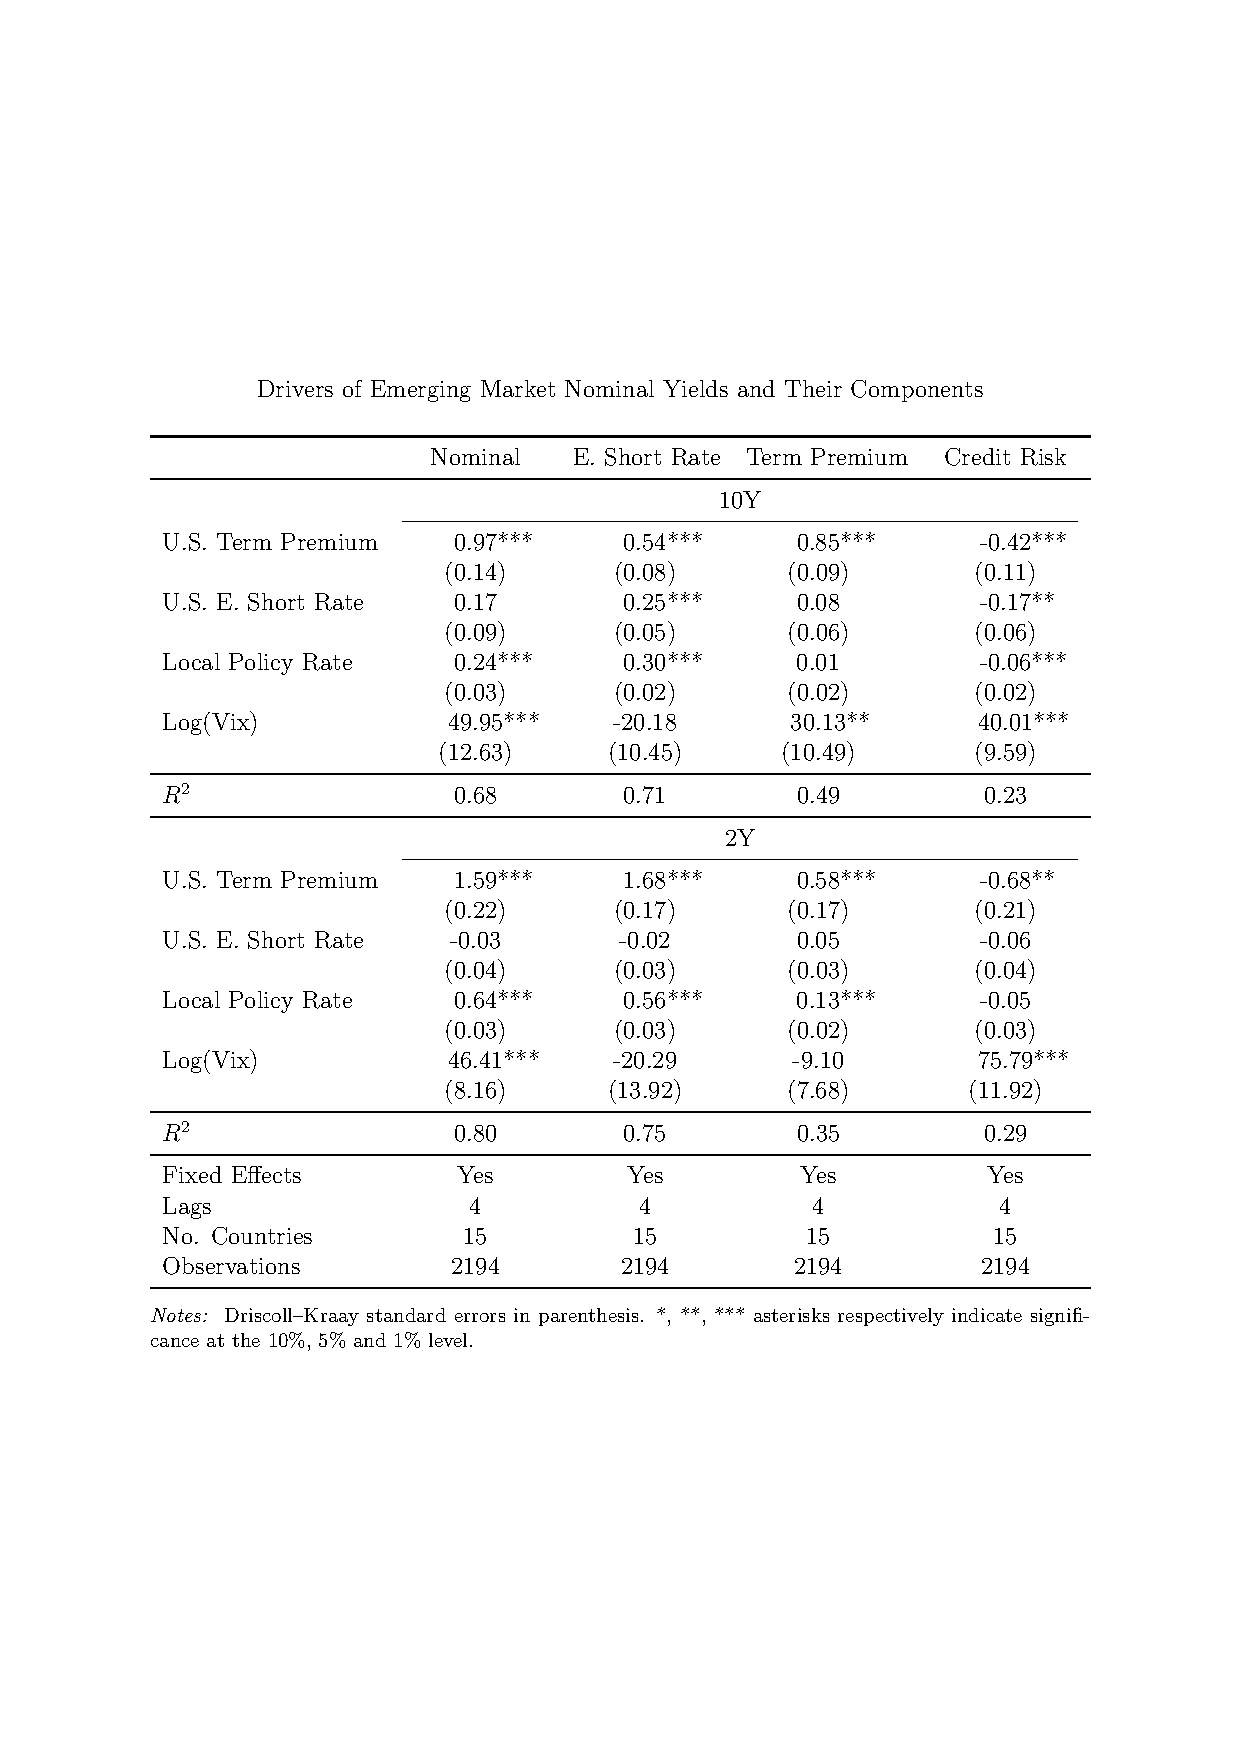
\includegraphics[trim={2cm 6.7cm 2cm 4cm},clip, width=0.95\textwidth,height=1.15\textheight]{../Tables/ycdcmp10y2y_v0.pdf}};
%	% \draw[step=0.5cm,gray,very thin] (-4,-4) grid (6,6);
%	\onslide<2>{
%		\draw[blue,thick] (-0.2,1.24) rectangle (1.2,1.7); %YP10Y
%		\draw[blue,thick] (-0.2,-1.49) rectangle (1.2,-1.02); %YP2Y
%		\draw[orange,thick] (-0.2,0.75) rectangle (1.2,1.21); %CBP10Y
%		\draw[orange,thick] (-0.2,-2) rectangle (1.2,-1.523); %CBP2Y
%	}
%	\onslide<3>{
%		\draw[blue,thick] (2,1.72) rectangle (3.5,2.19); % TP10Y
%		\draw[blue,thick] (2,-1.05) rectangle (3.5,-0.54); %TP2Y
%		\draw[orange,thick] (2,0.23) rectangle (3.5,0.74); % VIX10Y
%		\draw[orange,thick] (2,-2.52) rectangle (3.5,-2); %VIX2Y
%	}
%	\onslide<4>{
%		\draw[blue,thick] (-0.2,1.7) rectangle (1.2,2.2); %TP10Y
%		\draw[blue,thick] (-0.2,-1.05) rectangle (1.2,-0.54); %TP2Y
%		\draw[orange,thick] (-0.2,0.24) rectangle (1.2,0.74); % VIX10Y
%		\draw[orange,thick] (-0.2,-2.52) rectangle (1.2,-2); %VIX2Y
%	}
%	\end{tikzpicture}
%\end{center}
%\begin{textblock*}{5cm}(1.07\textwidth,0.175\textheight)
%	\hyperlink{Drivers10Y}{\beamergotobutton{10Y}}
%\end{textblock*}
%\begin{textblock*}{5cm}(1.07\textwidth,0.525\textheight)
%	\hyperlink{Drivers2Y}{\beamergotobutton{2Y}}
%\end{textblock*}
%\end{frame}

\begin{frame}[label=Drivers10Y2Y]
\vspace{-0.9cm} % \vspace{-2.2cm}
\begin{center}
	\begin{tikzpicture}
	\node (table) at (0,0)
	{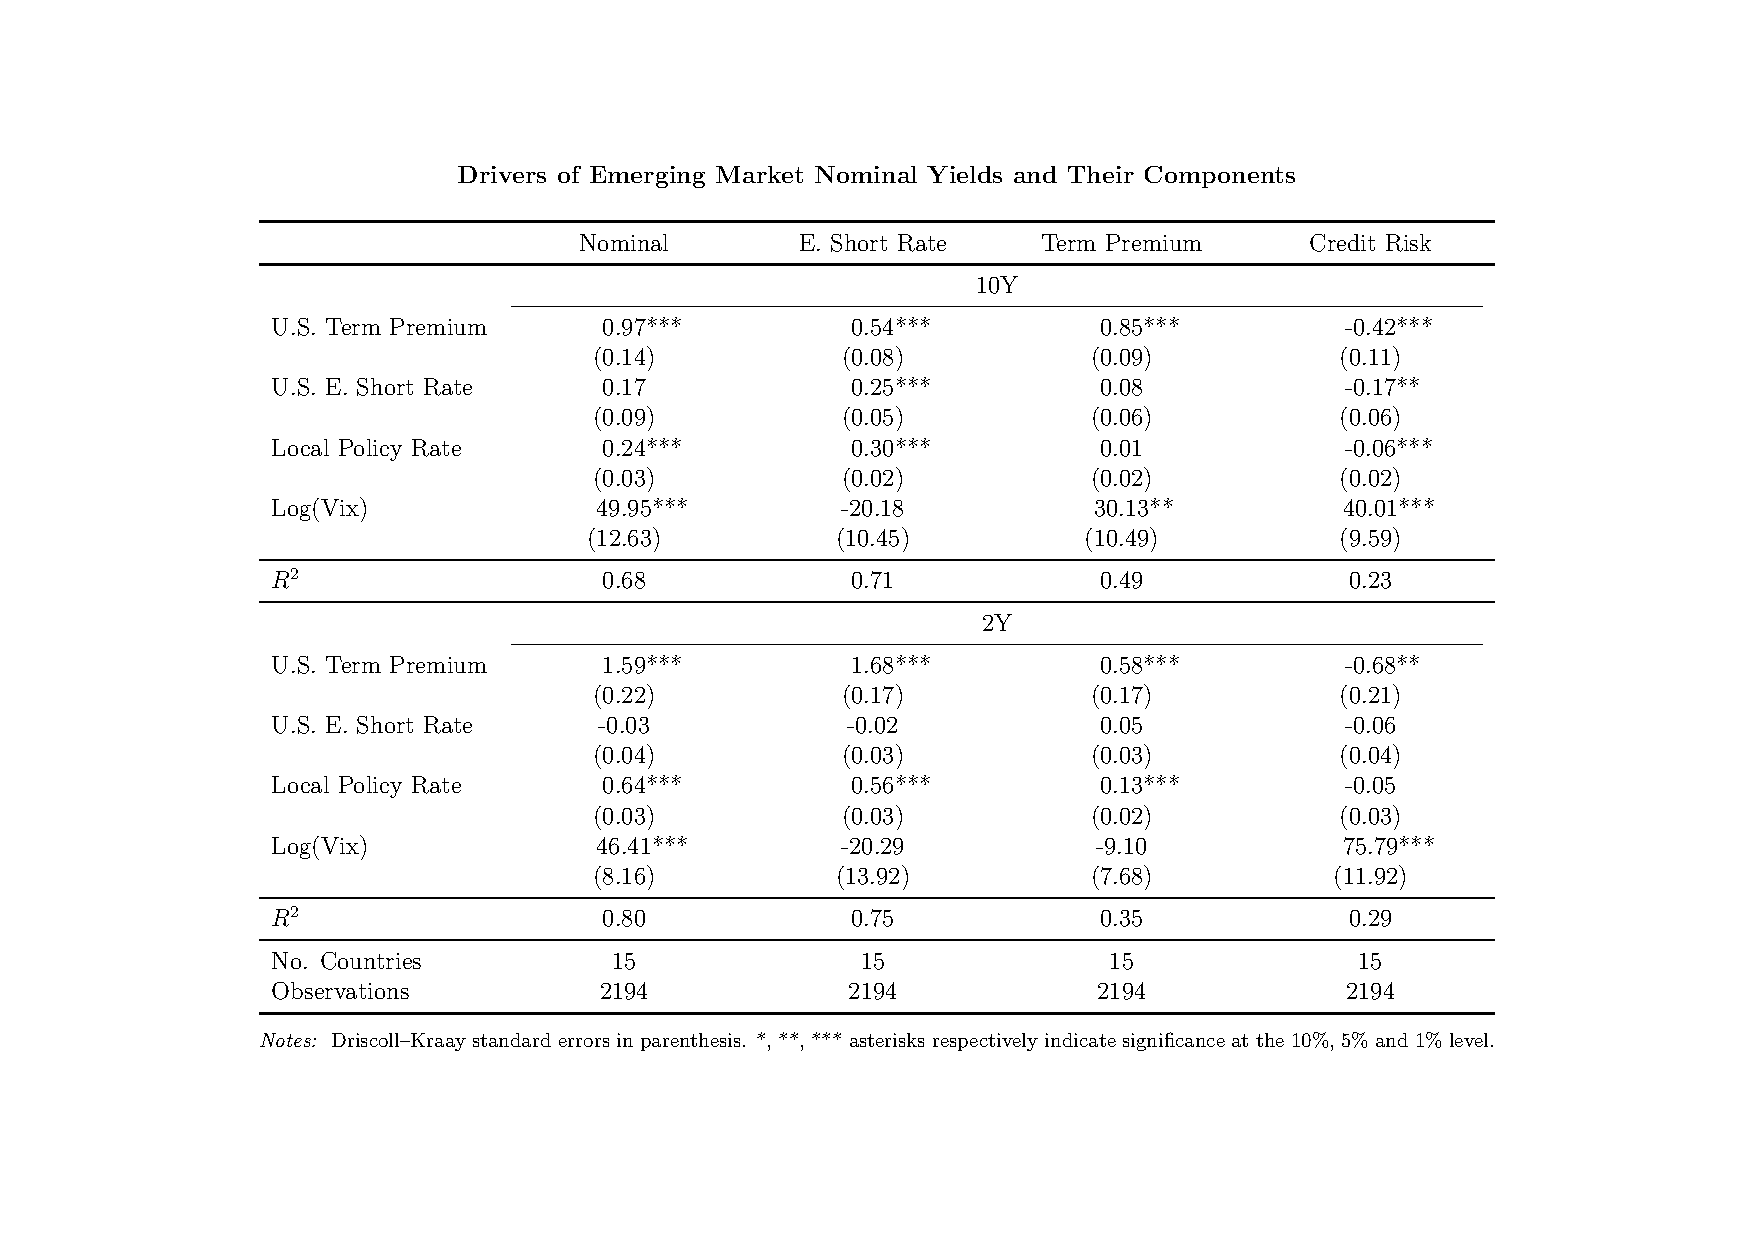
\includegraphics[trim={3cm 2cm 2.85cm 1cm},clip, width=1\textwidth,height=1.15\textheight]{../Tables/ycdcmp10y2y.pdf}};
	% \draw[step=0.5cm,gray,very thin] (-4,-4) grid (6,6);
	\onslide<2>{
		\draw[blue,thick] (-0.7,1.38) rectangle (0.55,1.88); %YP10Y blue
		\draw[blue,thick] (-0.7,-1.51) rectangle (0.55,-1.02); %YP2Y blue
		\draw[orange,thick] (-0.7,0.85) rectangle (0.55,1.34); %CBP10Y orange
		\draw[orange,thick] (-0.7,-2.05) rectangle (0.55,-1.55); %CBP2Y orange
	}
	\onslide<3>{
		\draw[blue,thick] (1.95,1.88) rectangle (3.25,2.38); % TP10Y blue
		\draw[blue,thick] (1.95,-1.03) rectangle (3.25,-0.51); %TP2Y blue
		\draw[orange,thick] (1.95,0.3) rectangle (3.25,0.85); % VIX10Y orange
		\draw[orange,thick] (1.95,-2.58) rectangle (3.25,-2.08); %VIX2Y orange
	}
	\onslide<4>{
		\draw[blue,thick] (-0.7,1.88) rectangle (0.55,2.38); %TP10Y
		\draw[blue,thick] (-0.7,-1.03) rectangle (0.55,-0.51); %TP2Y
		\draw[orange,thick] (-0.7,0.3) rectangle (0.55,0.85); % VIX10Y
		\draw[orange,thick] (-0.7,-2.58) rectangle (0.55,-2.08); %VIX2Y
	}
	\end{tikzpicture}
\end{center}
\begin{textblock*}{5cm}(1.07\textwidth,0.23\textheight)
	\hyperlink{Drivers10Y}{\beamergotobutton{10Y}}
\end{textblock*}
\begin{textblock*}{5cm}(1.07\textwidth,0.59\textheight)
	\hyperlink{Drivers2Y}{\beamergotobutton{2Y}}
\end{textblock*}
\end{frame}
\note{This table reports the estimated coefficients for the 2Y and 10Y nominal yields and their components. I want to highlight 3 things from this table in relation to the YC channel.}

\note{First, notice that the response of ESR to the domestic policy rate is stronger at the short end than at the long end. Also, the ESR is associated with its US counterpart only at the long end but not at the short end}
\note{This evidence shows that the monetary autonomy in EMs is stronger at the short end than at the long end.}

\note{The second point is that the response of the term premia in EMs to the US TP increases with maturity. Also, the term premia in EMs is positively associated with the VIX only at the long end.}
\note{This shows that the GFCy (represented here by the US TP and the VIX) is more relevant for LT yields than for ST ones.}

\note{The last point is that there are risk spillovers to the ESR in EMs from the US TP but not from the VIX. Those risk spillovers are stronger at the shor end than at the long end as suggested by Kalemli-Ozkan.}

\note{The results from this analysis are therefore in line with the implications of the YC channel.}
\note{Here, I am highilighting the evidence supporting the YC channel but in the paper, I discuss the effects of the other drivers not shown in this table.}


\note{In particular, the term premia in EMs is countercyclical, it raises during recessions.}

%\note{Higher TP during recessions: high UNE, low IP. Evidence of EM TP countercyclical.}
%\note{INF erodes value of nominal bonds: in periods of rising INF demand a higher TP.}
%\note{Higher TP due to FX depreciation in line with risk-taking channel of FX.
%	Currency depreciation tightens financial conditions, higher sovereign bond spreads.}
%\note{Effect of the domestic variables in line with findings for AEs. 
%	Investors demand a higher term premium during recessions, when the unemployment rate increases. This shows evidence of a countercyclical behavior of the TP in EMs.
%	The positive effect of inflation on the TP conforms with the idea that inflation erodes the value of nominal bonds and so in periods of rising inflation investors demand a higher TP.}
%\note{A depreciation of the LC is associated with an increase in the TP. This seems counterintuitive since EMs are usually commodity exporters so it appears to contradict the standard trade-channel effect. 
%	However, it is in line with the risk-taking channel of exchange rates found by \cite{HofmannShimShin:2017}, according to which currency depreciation is associated with tighter financial conditions and increased sovereign bond spreads.}


%{%
%	\setbeamertemplate{frame footer}{See \cite{Kuttner:2001,GSS:2005a,Swanson:2018,RogersScottiWright:2018}.}
\begin{frame}
\frametitle{U.S. Monetary Policy Surprises}

Asset price changes in 2-hour windows around FOMC meetings % since 2000
%Surprises:
	\begin{itemize}
		\item \alert{Target}: change in yield on federal funds futures \citep{Kuttner:2001}
		\item \alert{Forward guidance}: residual of change in yield for 8\(^{th}\) Eurodollar futures onto target surprise \citep{GSS:2005a}
		\item \alert{Asset purchases}: residual of change in yield of 10Y Treasury futures onto target and FG surprises \citep{Swanson:2018} % target and forward guidance surprises starting in 2009
	\end{itemize}
\begin{center}
%\documentclass[border=3pt,tikz]{standalone}
\usetikzlibrary{decorations.pathreplacing}

%\begin{document}

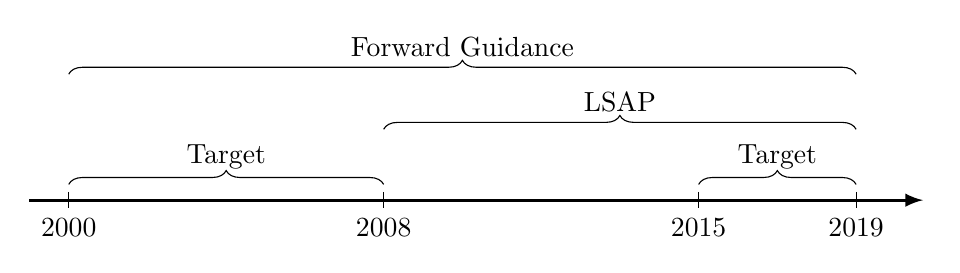
\begin{tikzpicture}
\draw[very thick,-{latex}] (0,0) -- (11.35,0) node{};
\foreach \x/\l in {0.5/2000,4.5/2008,8.5/2015,10.5/2019}
  \draw (\x,3pt) -- (\x,-3pt) node[below]{$\l$};
\draw [decorate,decoration={brace,amplitude=5pt}]
  (0.5,1.6) -- (10.5,1.6) node[midway,yshift=1em]{Forward Guidance};
\draw [decorate,decoration={brace,amplitude=5pt}]
  (4.5,0.9) -- (10.5,0.9) node[midway,yshift=1em]{LSAP};
\draw [decorate,decoration={brace,amplitude=5pt}]
 (0.5,0.2) -- (4.5,0.2) node[midway,yshift=1em]{Target};
\draw [decorate,decoration={brace,amplitude=5pt}]
 (8.5,0.2) -- (10.5,0.2) node[midway,yshift=1em]{Target};
\end{tikzpicture}

%\end{document}


%\begin{tikzpicture}
%\draw[very thick,-{latex}] (0,0) -- (11,0) node{};
%\foreach \x/\l in {0.5/2000,4.2/2008,5.2/2009,8.5/2015,10.5/2019}
%\draw (\x,3pt) -- (\x,-3pt) node[below]{$\l$};
%\draw [decorate,decoration={brace,amplitude=5pt}]
%(0.5,1.4) -- (10.5,1.4) node[midway,yshift=1em]{Forward Guidance};
%\draw [decorate,decoration={brace,amplitude=5pt}]
%(5.2,0.8) -- (10.5,0.8) node[midway,yshift=1em]{LSAP};
%\draw [decorate,decoration={brace,amplitude=5pt}]
%(0.5,0.2) -- (4.2,0.2) node[midway,yshift=1em]{Target};
%\draw [decorate,decoration={brace,amplitude=5pt}]
%(8.5,0.2) -- (10.5,0.2) node[midway,yshift=1em]{Target};
%\end{tikzpicture}

%Chronology of Fed’s Quantitative Easing & Tightening
%https://www.yardeni.com/chronology-of-feds-quantitative-easing/
\end{center}
%\begin{center}
%	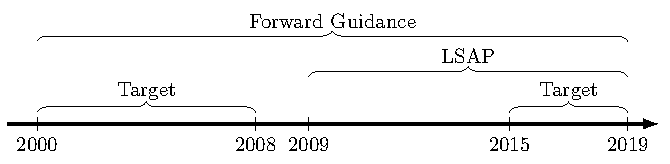
\includegraphics[trim={0cm 0cm 0cm 0cm},clip,width=0.85\textwidth,height=0.95\textheight]{../Figures/MPS/USMPtimeline}
%\end{center}
\end{frame}
%}
\note{The analysis so far has not identified US MP surprises and is not suitable to analyze the persistence of the effects.}
\note{To address that, I capture unexpected changes in the monetary stance in the US following the literature that identifies surprises in MP using intraday data on asset prices in 2-hour windows around FOMC meetings.}
\note{Since Fed's announcements provide different types of information, in the analysis I distinguish between three types of MP decisions.}
\note{Surprises about the target federal funds rate are based on the change in the yield on FFF contracts.}
\note{Surprises about the future path of the policy rate are equal to the residual from a regression of the change in the yield for the 8th Eurodollar futures contract onto the target surprise.}
\note{The 8th Eurodollar futures contract is a bet on the level of 3M interest rates about 2Y ahead. At the ZLB, this was around the shortest point on the YC that could be influenced by MP.}
\note{And finally, LSAP surprises are equal to the residual from a regression of the change in the yield of 10Y Treasury futures onto the target and FG surprises.}
\note{Notice that by construction the three types of surprises are uncorrelated.}
\note{A positive value in any of the surprises represents a tightening of the monetary stance, and a negative value represents an easing.}
\note{During the ZLB period there were essentially no target surprises. LSAP surprises only make sense after the GFC. And there have been FG surprises over the whole sample period.}

\begin{frame}
\frametitle{Measuring the Effects on EM Yields}
%\vspace{-1cm}
Panel local projections:

\vspace{-0.4cm}
\begin{equation*} \label{eq:uPanelLP}
	\eqpanelLP
\end{equation*}	% \ref{eq:nPanelLP}
%\vspace{-0.7cm}
\begin{itemize}
\item \(\yld_{\idxspnl}\): 10Y and 2Y EM nominal \alert{yields} and their \alert{components}
\item \(\idxh = 0, 1, \ldots, 45\) days
\item \(\alpha_{\idxh,\idxi}\): country fixed effects
\item \(\epsilon^{j}_{\idxt}\): \alert{three} types of monetary policy \alert{surprises}
\item \(\fx_{\idxspnllag}\): one-day lag in the exchange rate
\end{itemize}
\end{frame}
\note{To quantify the effects of US MP on EM yields, I use panel local projections for the daily changes in the nominal yields and their components, which allow me to estimate the effects on the day of a surprise as well as their persistence.}
\note{I control for the lag of the dependent variable and the lag of the FX to rule out explanations of yield changes due to the exchange rate.}
\note{Since the Fed has been more aggressive stimulating the economy over the sample period, all responses are assessed relative to a 1 basis point easing surprise.}


\note{Large number of daily observations reduces the potential for Nickell bias. Responses are essentially the same when I removed the lag of the depvar.}
%\note{Keep in mind that since there are two curves, it is important to understand the effects on both curves when interpreting the results.}


\begin{frame}[label=TargetEM]
\frametitle{Effects of Target Easing on EM Yields}
\begin{figure}[!htbp]
\begin{center} % trim removes: left, down, right, top
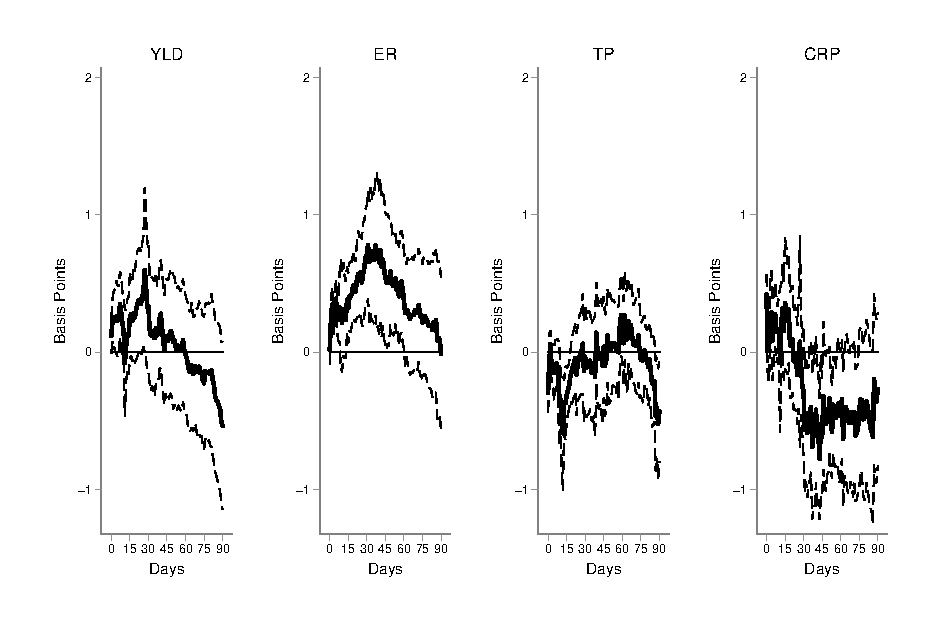
\includegraphics[trim={0cm 0cm 0cm 0cm},clip,height=0.45\textheight,width=0.85\linewidth]{../Figures/LPs/LagDep-FX/Target/EM/TargetEMnomyptpphi120m.eps}
\par\end{center}
\end{figure}
\vspace{-0.5cm}
\begin{figure}[!htbp]
\begin{center} % trim removes: left, down, right, top
\includegraphics[trim={0cm 0cm 0cm 0.76cm},clip,height=0.45\textheight,width=0.85\linewidth]{../Figures/LPs/LagDep-FX/Target/EM/TargetEMnomyptpphi24m.eps}
\par\end{center}
\end{figure}
\begin{textblock*}{8mm}(10mm,30mm)
\small \textbf{10Y}
\end{textblock*}
\begin{textblock*}{8mm}(10mm,65mm)
\small \textbf{2Y}
\end{textblock*}
\begin{textblock*}{5cm}(1.07\textwidth,0.65\textheight)
\hyperlink{TargetUS}{\beamergotobutton{US}}
\end{textblock*}
\end{frame}
\note{This figure shows the responses of the 2Y and 10Y nominal yields and their components to a 1 basis point target easing surprise.}
\note{Red arrows indicate the responses on the day of the surprise.}
%\note{The dotted lines are 90\% confidence bands.} %computed using the DK SE

\note{Following a target easing surprise, the YCs of EMs steepen since ST yields decline by more. Also notice that the response builds over time, which can be attributed to slow-moving capital.}
\note{The response of the US YC is similar. It also steepens over time.}

\note{Looking at the effects on the components, we can see that investors expect CBs in EMs to follow the monetary stance of the Fed, in this case an easing of financial conditions, with the effect being somewhat stronger at the short end.}
\note{In fact, most of the effect of a target surprise is reflected on the ESR component. There is essentially no effect on the term premia and on the CRC at the short end. However, the CRC at the lond end increases one month after the surprise.}
\note{Mechanically, this result suggests that investors reallocate capital into US Treasuries along the YC but only into EM sovereign bonds at the short end which increases the nominal-synthetic spread at the long end.}
\note{The economic intuition behind this result can be related to the reason why EMs default in the first place. The decline in the ESR might lead to an eventual depreciation of the LC, which would have a negative effect on the balance sheet of firms with assets in LC but liabilities in FC. Different papers have indeed documented that the corporate sector in EMs has increased its borrowing in FC over time.}
\note{A large depreciation of the LC might therefore trigger corporarte defaults that would negatively affect domestic output. In such a case, a sovereign default would be preferred to a depreciation, increasing the price of bearing credit risk.}
\note{Du and Schreger document support for this mechanism.}
\note{Notice that the effect is not expected in the short term, since the CRC increases only for LT yields.}
\note{This can be seen as the fiscal implications in EMs of MP in the US.}


\begin{frame}[label=FGEMpre]
\frametitle{Effects of Forward Guidance Easing on EM Yields: Pre-GFC}
\begin{figure}[!htbp]
	\begin{center} % trim removes: left, down, right, top
		\includegraphics[trim={0cm 0cm 0cm 0cm},clip,height=0.45\textheight,width=0.85\linewidth]{../Figures/LPs/LagDep-FX/Path/EM/PathEMnomyptpphi120mPre.eps}
		\par\end{center}
\end{figure}
\vspace{-0.5cm}
\begin{figure}[!htbp]
	\begin{center} % trim removes: left, down, right, top
		\includegraphics[trim={0cm 0cm 0cm 0.76cm},clip,height=0.45\textheight,width=0.85\linewidth]{../Figures/LPs/LagDep-FX/Path/EM/PathEMnomyptpphi24mPre.eps}
		\par\end{center}
\end{figure}
\begin{textblock*}{8mm}(10mm,30mm)
	\small \textbf{10Y}
\end{textblock*}
\begin{textblock*}{8mm}(10mm,65mm)
	\small \textbf{2Y}
\end{textblock*}
\begin{textblock*}{5cm}(1.07\textwidth,0.65\textheight)
	\hyperlink{FGUSpre}{\beamergotobutton{US}}
\end{textblock*}
\end{frame}
\note{The literature documents that US MP spillovers to EM yields changed after the GFC, so I present the responses to a FG easing surprise before and after the GFC.}

\note{As you can see in this figure, before 2008, a FG easing surprise led to a downward parallel shift in EM YCs in the month following the surprise, which was mainly driven by a parallel decline in term premia since the ESR and the CRC essentially did not respond.}
\note{The sluggish response that I mentioned for target surprises can also be seen here.}

\note{The effect on US yields is not as clear as for EM yields but FG easing surprises also reduce the US term premium, with the effect being somewhat stronger at the long end.}

%\note{Slightly reduced CRC on impact.}


\begin{frame}[label=FGEMpost]
\frametitle{Effects of Forward Guidance Easing on EM Yields: Post-GFC}
\begin{figure}[!htbp]
\begin{center} % trim removes: left, down, right, top
\includegraphics[trim={0cm 0cm 0cm 0cm},clip,height=0.45\textheight,width=0.85\linewidth]{../Figures/LPs/LagDep-FX/Path/EM/PathEMnomyptpphi120mPost.eps}
\par\end{center}
\end{figure}
\vspace{-0.5cm}
\begin{figure}[!htbp]
\begin{center} % trim removes: left, down, right, top
\includegraphics[trim={0cm 0cm 0cm 0.76cm},clip,height=0.45\textheight,width=0.85\linewidth]{../Figures/LPs/LagDep-FX/Path/EM/PathEMnomyptpphi24mPost.eps}
\par\end{center}
\end{figure}
\begin{textblock*}{8mm}(10mm,30mm)
\small \textbf{10Y}
\end{textblock*}
\begin{textblock*}{8mm}(10mm,65mm)
\small \textbf{2Y}
\end{textblock*}
\begin{textblock*}{5cm}(1.07\textwidth,0.65\textheight)
\hyperlink{FGUSpost}{\beamergotobutton{US}}
\end{textblock*}
\end{frame}
\note{This figures shows the responses of EM yields to a FG easing surprise after the GFC.}

\note{For the UMPs, let me also show you the responses of US yields.}
\note{The figure shows the responses of US yields to a FG easing surprise after the GFC.}
\note{Notice that the effect is stronger on LT yields, it is persistent and it is mainly driven by the term premium.}
\note{In fact, one of the goals of the Fed of making announcements about the future path of the federal funds rate after the GFC was to reduce LT yields in the US mainly by reducing the term premium.}

\note{In the case of EMs, the effect on LT yields is shorter than in US yields. Therefore, the nominal-synthetic spread in EM yields widens at the long end. The same economic intuition applied with target surprises is still valid for FG surprises. That is, the effect of an eventual depreciation of the LC on the balance sheet of the corporate sector increases the price of bearing credit risk.} %makes investors relatively more willing to invest in LT bonds in the US than in EM

\note{You can also see that the response of the term premia at the lond end is similar in EMs than in the US. In other words, announcements by the Fed about the future path of the federal funds rate aimed at reducing the term premium in US yields at the long end, also reduce the term premia in EM yields at the long end.}
\note{This is where accounting for credit risk pays off because if it were to be ignored, one would conclude that unconventional policies do not affect the term premia in EMs. And the reason is that the `clean' term premium that I propose and the CRC part respond in opposite directions with magnitudes that almost offset each other, so there is no net effect in the term premium contaminated with credit risk.}

\note{In relation to the YC channel, a FG easing surprise not only reduces the term premium in EMs at the long end but also the expectation for the policy rates at the short end.}
\note{This is consistent with the risk spillovers mechanism highlighted before.}


\begin{frame}[label=LSAPEM]
\frametitle{Effects of Asset Purchase Easing on EM Yields}
\begin{figure}[!htbp]
\begin{center} % trim removes: left, down, right, top
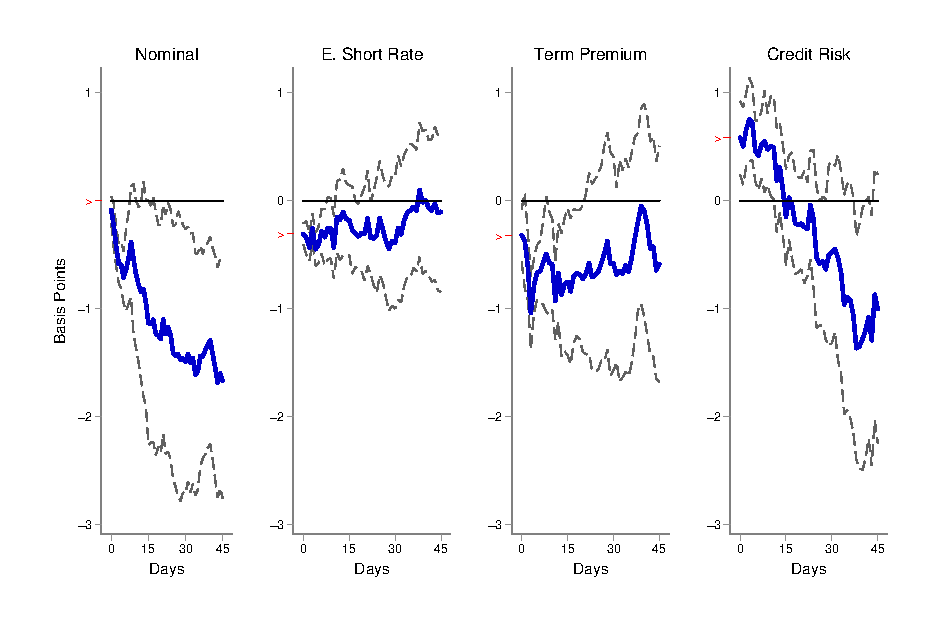
\includegraphics[trim={0cm 0cm 0cm 0cm},clip,height=0.45\textheight,width=0.85\linewidth]{../Figures/LPs/LagDep-FX/LSAP/EM/LSAPEMnomyptpphi120m.eps}
\par\end{center}
\end{figure}
\vspace{-0.5cm}
\begin{figure}[!htbp]
\begin{center} % trim removes: left, down, right, top
\includegraphics[trim={0cm 0cm 0cm 0.76cm},clip,height=0.45\textheight,width=0.85\linewidth]{../Figures/LPs/LagDep-FX/LSAP/EM/LSAPEMnomyptpphi24m.eps}
\par\end{center}
\end{figure}
\begin{textblock*}{8mm}(10mm,30mm)
\small \textbf{10Y}
\end{textblock*}
\begin{textblock*}{8mm}(10mm,65mm)
\small \textbf{2Y}
\end{textblock*}
\begin{textblock*}{5cm}(1.07\textwidth,0.65\textheight)
\hyperlink{LSAPUS}{\beamergotobutton{US}}
\end{textblock*}
\end{frame}
\note{This last figure shows the effects on EM yields to announcements about asset purchases.}

\note{Let me also refer to the response of US yields to those surprises.}
\note{An asset purchase easing surprise flattens the US YC since the effect is stronger on LT yields than on ST ones. In particular notice that the response of LT yields is more than 1-to-1, and that the surprises reduce both the ESR and the TP at short and long maturities.}

\note{In the case of EMs, asset purchase easing surprises also flatten their YCs but the effect lasts longer on EM yields than on US yields. Therefore, an asset purchase surprise more clearly incentivizes investors to *eventually* hold LT bonds in EMs than target and FG surprises.}
\note{This effect reduces the term premium and the CRC.}
\note{This on-impact increase in the CRC at the long end, however, seems to be more a reflection of the response in the US Treasuries market than on the bond markets in emerging economies.}

\note{Similar to the responses to a FG easing surprise after the GFC, an asset purchase easing surprise not only reduces the term premium in EMs at the long end but also the expectation for the policy rates at the short end.}
\note{This evidence also confirms the results I mentioned before about a YC channel.}
\note{In particular, the UMPs, namely FG and asset purchases, implemented by the Fed after the GFC transmit to EM yields through their different components, which can limit the influence central banks in EMs can exert over their domestic YCs.}


\section{Conclusions}
\note{Let me now conclude.}

\begin{frame}
\frametitle{Conclusions}

\textbf{Three}-part decomposition of EM sovereign yields
\begin{itemize}
\item Average expected short rates \item Term premium \item \alert{Credit risk} compensation
\end{itemize}

U.S. monetary policy \textbf{spillovers} to EM sovereign yields
\begin{enumerate}
\item Responses are economically \alert{significant} yet \alert{delayed}
\item Reassessment of policy rate expectations and repricing of \alert{risks}
\item Evidence of a \alert{yield curve channel} since 2008
\end{enumerate}
\end{frame}
\note{I propose a 3-part decomposition of the sovereign bond yields of EMs that explicitly takes into account the risk that those countries might default on their LC debt.}
\note{I then use this decomposition to characterize the transmission channels of US MP.}
\note{I find that the responses of EM yields to surprises in US MP are economically significant but they are delayed over the month following a surprise.}
\note{Also, surprises in US MP lead to a reassessment of policy rate expectations and a repricing not only of interest risk but also of credit risk in EMs.}
\note{Finally, the UMPs implemented by the Fed after the GFC limit the influence central banks in EMs can exert over their domestic YCs.}

\note{A final takeaway from the paper is that it is important to explicitly account for credit risk in the LC debt of EMs and to examine the effects at different maturities to adequately characterize the transmission channels of US MP.}
\note{I am happy to take any other question.}


%\note{These results have implications for both AE and EM.}
%\note{These results give rise to further research questions like, for example, what tools do CBs in EM have at their disposal to deal with MP spillovers from abroad.}
%\note{Extensions: nominal-real decompositions, jumps.}
%\note{YC channel: EM monetary autonomy decreases along the yield curve and involves the CRC.}


\begin{frame}[standout]
Appendix
\end{frame}

\appendix

\begin{frame}[label=CreditRating]
\frametitle{Credit Risk in Local Currency Yields}
\begin{center}
	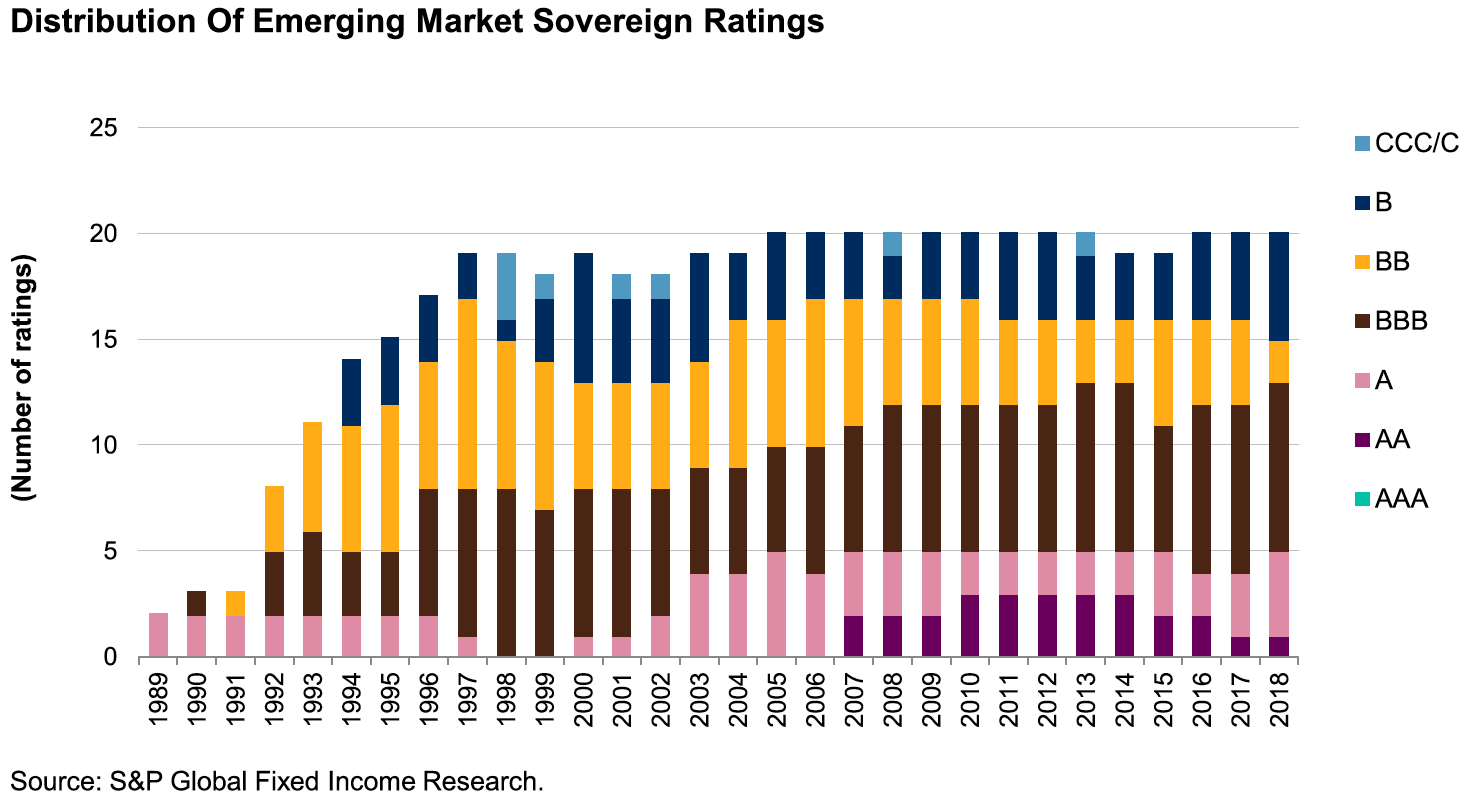
\includegraphics[width=0.95\textwidth,height=0.9\textheight]{../Figures/Slides/EM_LC_Ratings.png}
\end{center}
\begin{textblock*}{5cm}(0.87\textwidth,1.06\textheight)
	\hyperlink{SovereignDefaults}{\beamerreturnbutton{Sovereigns Defaults}}
\end{textblock*}
\end{frame}
\note{Few EM have a credit rating of A and more than 30 have a rating below investment grade of BBB.}
\note{Figure: include Argentina, Brazil, China, Colombia, Egypt, Hungary, India, Indonesia, Lebanon, Malaysia, Mexico, Pakistan, Philippines, Poland, Qatar, Russia, Saudi Arabia, South Africa, Thailand, Turkey.}
\note{A bond is considered investment grade if its credit rating is BBB- or higher. Bonds rated BB+ and below are considered to be speculative grade.}
\note{Countries w/ AAA ratings: Australia, Canada,	Denmark, Finland, Germany, Luxembourg, Netherlands, Norway, Singapore, Sweden, Switzerland.}
\note{BRL, TRY, ZAR don't have investment grade.}
%\note{Credit risk broadly defined: (selective) default risk, currency convertibility risk, regulation risk, capital controls, jurisdiction risks, liquidity risk, sovereign restructurings.}


\begin{frame}[label=YldStats]
\frametitle{Descriptive Statistics}
\begin{figure}[!htbp]
	\begin{center} % trim removes: left, down, right, top
		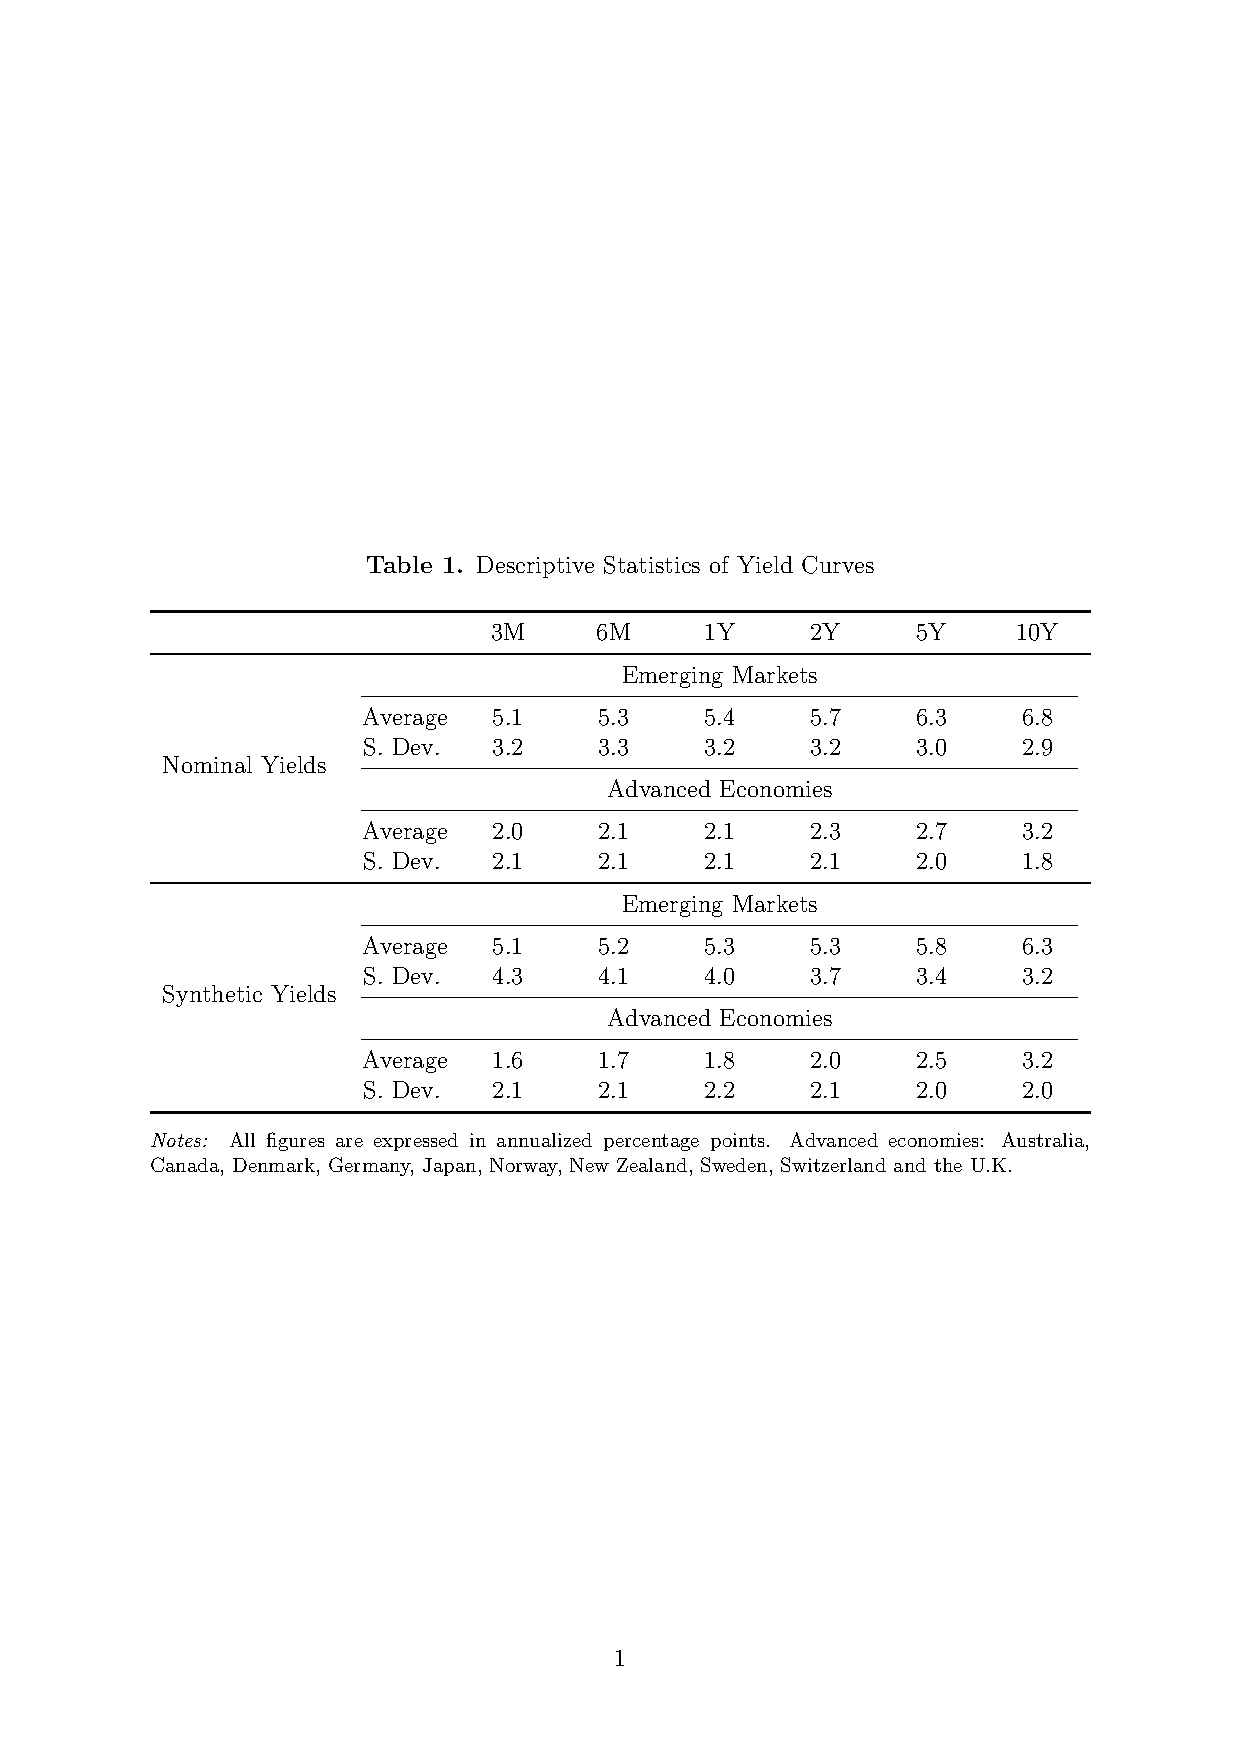
\includegraphics[trim={2.5cm 7.5cm 2.5cm 10cm},clip, width=0.95\textwidth,height=1.05\textheight]{../Tables/yldcrvstats.pdf}
		\par\end{center}
\end{figure}

\begin{textblock*}{3cm}(1.02\textwidth,.18\textheight)
	\hyperlink{YldData}{\beamerreturnbutton{Yield Data}}
\end{textblock*}
\end{frame}
\note{Table reports descriptive statistics for different tenors of the nominal and synthetic YC for the EM and includes those from AE for comparison.}
\note{YCs exhibit standard properties such as an upward slope.}
\note{In general interest rates in EM are higher than in AE, the table reflects that.}

\note{For instance, the level and the volatility of EM curves are larger than those of AE.} 
\note{Also, the short end of their curves is more volatile than the long end, particularly so for the synthetic curve.}
\note{Higher volatility at ST makes the model's fit at ST harder. Don't affect the results b/c the analysis focuses on the 2Y and 10Y.}
\note{10 AEs: AUD, CAD, CHF, DKK, EUR, GBP, JPY, NOK, NZD, SEK}


\begin{frame}[label=AssetPricing]
\frametitle{Asset Pricing}
Under no arbitrage \(\rightarrow\) \(\exists\) a stochastic discount factor \(\SDF > 0\)
\newline

\(\SDF\) prices all nominal bonds under probability measure \(\Pmeasure\)
\begin{equation*} \label{eq:uPzeroP}
	\PzeroP 
\end{equation*}
\vspace{1pt}

\(\SDF\) \(\rightarrow\) \(\exists\) a risk-neutral measure \(\Qmeasure\) defined as % theoretical risk-neutral pricing
\begin{equation*} \label{eq:uPzeroQ}
	\PzeroQ 
\end{equation*}

\begin{textblock*}{3cm}(1\textwidth,1.05\textheight)
	\hyperlink{ATSMsummary}{\beamerreturnbutton{Overview}}
\end{textblock*}
\end{frame}
\note{Theoretical measure under which hypothetical investors are risk neutral that also serves to price bonds.}


\begin{frame}[label=SDF]
\frametitle{Stochastic Discount Factor}
Stochastic discount factor
\begin{equation*} \label{eq:uSDF}
	\eqSDF 
\end{equation*}

Market prices of risk
\begin{equation*} \label{eq:uRiskprice}
	\eqriskprice 
\end{equation*}

One-period interest rate
\begin{equation*} \label{eq:uShortRate}
	\eqshortrate 
\end{equation*}

\begin{textblock*}{3cm}(1\textwidth,1.05\textheight)
	\hyperlink{ATSMsummary}{\beamerreturnbutton{Overview}}
\end{textblock*}

\end{frame}
\note{The model specifies the SDF as a function of the one-period interest rate and the market prices of risk, which are in turn affine functions of the pricing factors}
\note{Market prices of risk control the transformation between the Q and P measures.}


\begin{frame}[label=BondPrices]
\frametitle{Bond Pricing}
Pricing factors under \(\Pmeasure\) measure % physical
\begin{equation*} \label{eq:uXvarsP}
	\eqXvarsFwdP
\end{equation*}

Bond prices % is an exponentially affine function of the pricing factors
\begin{equation*}
	\Pzero = \exp\left( \affineA + \affineB \Xvars \right) ,
\end{equation*}

\begin{center}
\(\affineA = A(\deltazero, \deltaone, \XmuP, \XPhiP, \XSigma, \tnr)\), \(\affineB = \mathcal{B}(\deltaone, \XPhiP, \tnr)\) % \(\affineAP = - \frac{1}{\tnr} \affineA\), \(\affineBP = - \frac{1}{\tnr} \affineB\), 
\end{center}

Pricing factors under \(\Qmeasure\) measure % risk-neutral
\begin{equation*} \label{eq:uXvarsQ}
	\eqXvarsFwdQ 
\end{equation*}

\begin{textblock*}{3cm}(1\textwidth,1.05\textheight)
\hyperlink{ATSMsummary}{\beamerreturnbutton{Overview}}
\end{textblock*}
\end{frame}
\note{Pricing factors are assumed to follow a first-order VAR.}
\note{These assumptions imply that the log price of the bond is an affine function of the pricing factors.}
\note{Coefficients are functions of the model's parameters and the maturity of the bond.}
\note{The structure for the market prices of risk implies that the dynamics of the pricing factors under the risk-neutral measure also follow a first-order VAR.}


\begin{frame}[label=SvyAugModel]
\frametitle{Survey-Augmented Model}

Expected average short rate % under \(\Pmeasure\)
\begin{equation*}
	\yZeroE = \frac{1}{\tnr} \ExpP \left[ \sum_{j=0} ^{\tnr-1} \srate_{\idxt+j} \right] = \affineAe + \affineBe \Xvars,
\end{equation*}
\vspace{3pt}

Forward rate from \(\tnr\) to \(\tnrfwd\) periods hence
\begin{equation*}
	\yZeroEfwd = \affineAeFwd + \affineBeFwd \Xvars.
\end{equation*}

\begin{textblock*}{3cm}(1\textwidth,1.05\textheight)
	\hyperlink{ATSMsummary}{\beamerreturnbutton{Overview}}
\end{textblock*}

\end{frame}
\note{To incorporate surveys in the model, the expected avg SR in the model is matched to the 5-year ahead implied forecast.}
\note{The LT implied forecast is matched to the 5Y forward 5Y hence.}


\begin{frame}[label=YldCBP]
%	\frametitle{Components: Expected Future Short Rate}
\begin{center}							% center the figure inside the minipage
	\includegraphics[trim={0cm 0cm 0cm 0cm},clip,height=0.95\textheight,width=\linewidth]{../Figures/Data/YLD10Y_CBP.eps} \\
\end{center}
\begin{textblock*}{15cm}(2.5mm,3mm)
	\textbf{10Y}
\end{textblock*}
\begin{textblock*}{5cm}(0.97\textwidth,1.05\textheight)
	\hyperlink{SCBP}{\beamerreturnbutton{Survey Data}}
\end{textblock*}
\end{frame}
\note{To see how sensible the implied forecasts for the short rate are, I compare them against the synthetic yields.}
\note{In this figure forecasts in orange and synthetic yields in blue. You can see that the magnitudes are comparable.}
\note{I compare them also against the real yields from TIPS and against an alternative approach using Taylor-rule type regressions, which also use forecasts for real GDP. The results are also comparable.}


\begin{frame}[label=YldDcmp10]
%	\frametitle{Decomposition of EM Nominal Yields}
\begin{center}							% center the figure inside the minipage
	\includegraphics[trim={0cm 0cm 0cm 0cm},clip,height=0.95\textheight,width=\linewidth]{../Figures/Estimation/ny_dcmp.eps} \\
\end{center}
\begin{textblock*}{15cm}(2.5mm,3mm)
	\textbf{10Y}
\end{textblock*}
\begin{textblock*}{5cm}(0.92\textwidth,1.07\textheight)
	\hyperlink{YldDcmp2}{\beamerreturnbutton{Decomposition HUF-MXN}}
\end{textblock*}
\end{frame}

%\begin{frame}[label=yPscbp]
%%	\frametitle{Components: Expected Future Short Rate}
%\vspace{0.1cm}
%\begin{center}							% center the figure inside the minipage
%	\includegraphics[trim={0cm 0cm 0cm 0cm},clip,height=0.95\textheight,width=\linewidth]{../Figures/Estimation/bsl_yP_scbp.eps} \\
%\end{center}
%\begin{textblock*}{15cm}(2.5mm,3mm)
%	\textbf{10Y}
%\end{textblock*}
%\begin{textblock*}{5cm}(0.97\textwidth,1.05\textheight)
%	\hyperlink{YldDcmp10}{\beamerreturnbutton{Decomposition}}
%\end{textblock*}
%\end{frame}

\begin{frame}[label=tpCI]
%	\frametitle{Components: Term Premium}
\begin{center}							% center the figure inside the minipage
\includegraphics[trim={0cm 0cm 0cm 0cm},clip,height=0.95\textheight,width=\linewidth]{../Figures/Estimation/bsl_tp_CI_10y_V1.eps} \\
\end{center}
\begin{textblock*}{15cm}(2.5mm,3mm)
	\textbf{10Y}
\end{textblock*}
\begin{textblock*}{5cm}(0.97\textwidth,1.05\textheight)
\hyperlink{YldDcmp10}{\beamerreturnbutton{Decomposition}}
\end{textblock*}
\end{frame}
\note{Survey-Based Term Premium Estimates}
\note{EM TP are time-varying.}
\note{Sensible TP estimates, mostly positive; fluctuate between 0\% and 5\%.}
\note{Sometimes they comove.}

\begin{frame}[label=crcCI]
%\frametitle{Components: Credit Risk Compensation}
\begin{center}							% center the figure inside the minipage
\includegraphics[trim={0cm 0cm 0cm 0cm},clip,height=0.95\textheight,width=\linewidth]{../Figures/Estimation/bsl_cr_CI_10y_V1.eps} \\
\end{center}
\begin{textblock*}{15cm}(2.5mm,3mm)
	\textbf{10Y}
\end{textblock*}
\begin{textblock*}{5cm}(0.97\textwidth,1.05\textheight)
\hyperlink{YldDcmp10}{\beamerreturnbutton{Decomposition}}
\end{textblock*}
\end{frame}

%\begin{frame}[label=rrtLT]
%%	\frametitle{Components: Expected Future Short Rate}
%\begin{center}							% center the figure inside the minipage
%	\includegraphics[trim={0cm 0cm 0cm 0cm},clip,height=1.05\textheight,width=\linewidth]{../Figures/Estimation/rrt_LTvsUSrrt.eps} \\
%\end{center}
%\begin{textblock*}{5cm}(0.95\textwidth,1.05\textheight)
%	\hyperlink{yPscbp}{\beamerreturnbutton{Model vs Forecasts}}
%\end{textblock*}
%\end{frame}

\begin{frame}[label=DYindex]
\frametitle{EM Yields Comovement}
\begin{figure}[!htbp]
	\begin{center} % trim removes: left, down, right, top
		\includegraphics[trim={0cm 0cm 0cm 0cm},clip,height=0.8\textheight,width=0.85\linewidth]{../Figures/Estimation/dy_index_dn_data.eps}
		\par\end{center}
\end{figure}
\begin{textblock*}{10cm}(45mm,83mm)
	\footnotesize Connectedness Index \citep{DieboldYilmaz:2014}
\end{textblock*}
\begin{textblock*}{5cm}(1.02\textwidth,0.55\textheight)
	\hyperlink{RollingCorr}{\beamergotobutton{Rolling Corr.}}
\end{textblock*}
\end{frame}

%\begin{frame}[label=RollingCorr]
%\frametitle{EM Yields Comovement}
%\begin{figure}[!htbp]
%\begin{center} % trim removes: left, down, right, top
%	\includegraphics[trim={0cm 0cm 0cm 0cm},clip,height=0.8\textheight,width=0.85\linewidth]{../Figures/Estimation/rolling_dn_data.eps}
%	\par\end{center}
%\end{figure}
%\begin{textblock*}{10cm}(67.5mm,83mm)
%\footnotesize Rolling Correlations
%\end{textblock*}
%\begin{textblock*}{5cm}(1.02\textwidth,0.55\textheight)
%\hyperlink{DYindex}{\beamergotobutton{D-Y Index}}
%\end{textblock*}
%\end{frame}


\begin{frame}[label=Drivers10Y]
%	\frametitle{EM Term Premium and Inflation Uncertainty}
\vspace{-0.8cm}
\begin{figure}[!htbp]
	\begin{center} % trim removes: left, down, right, top
		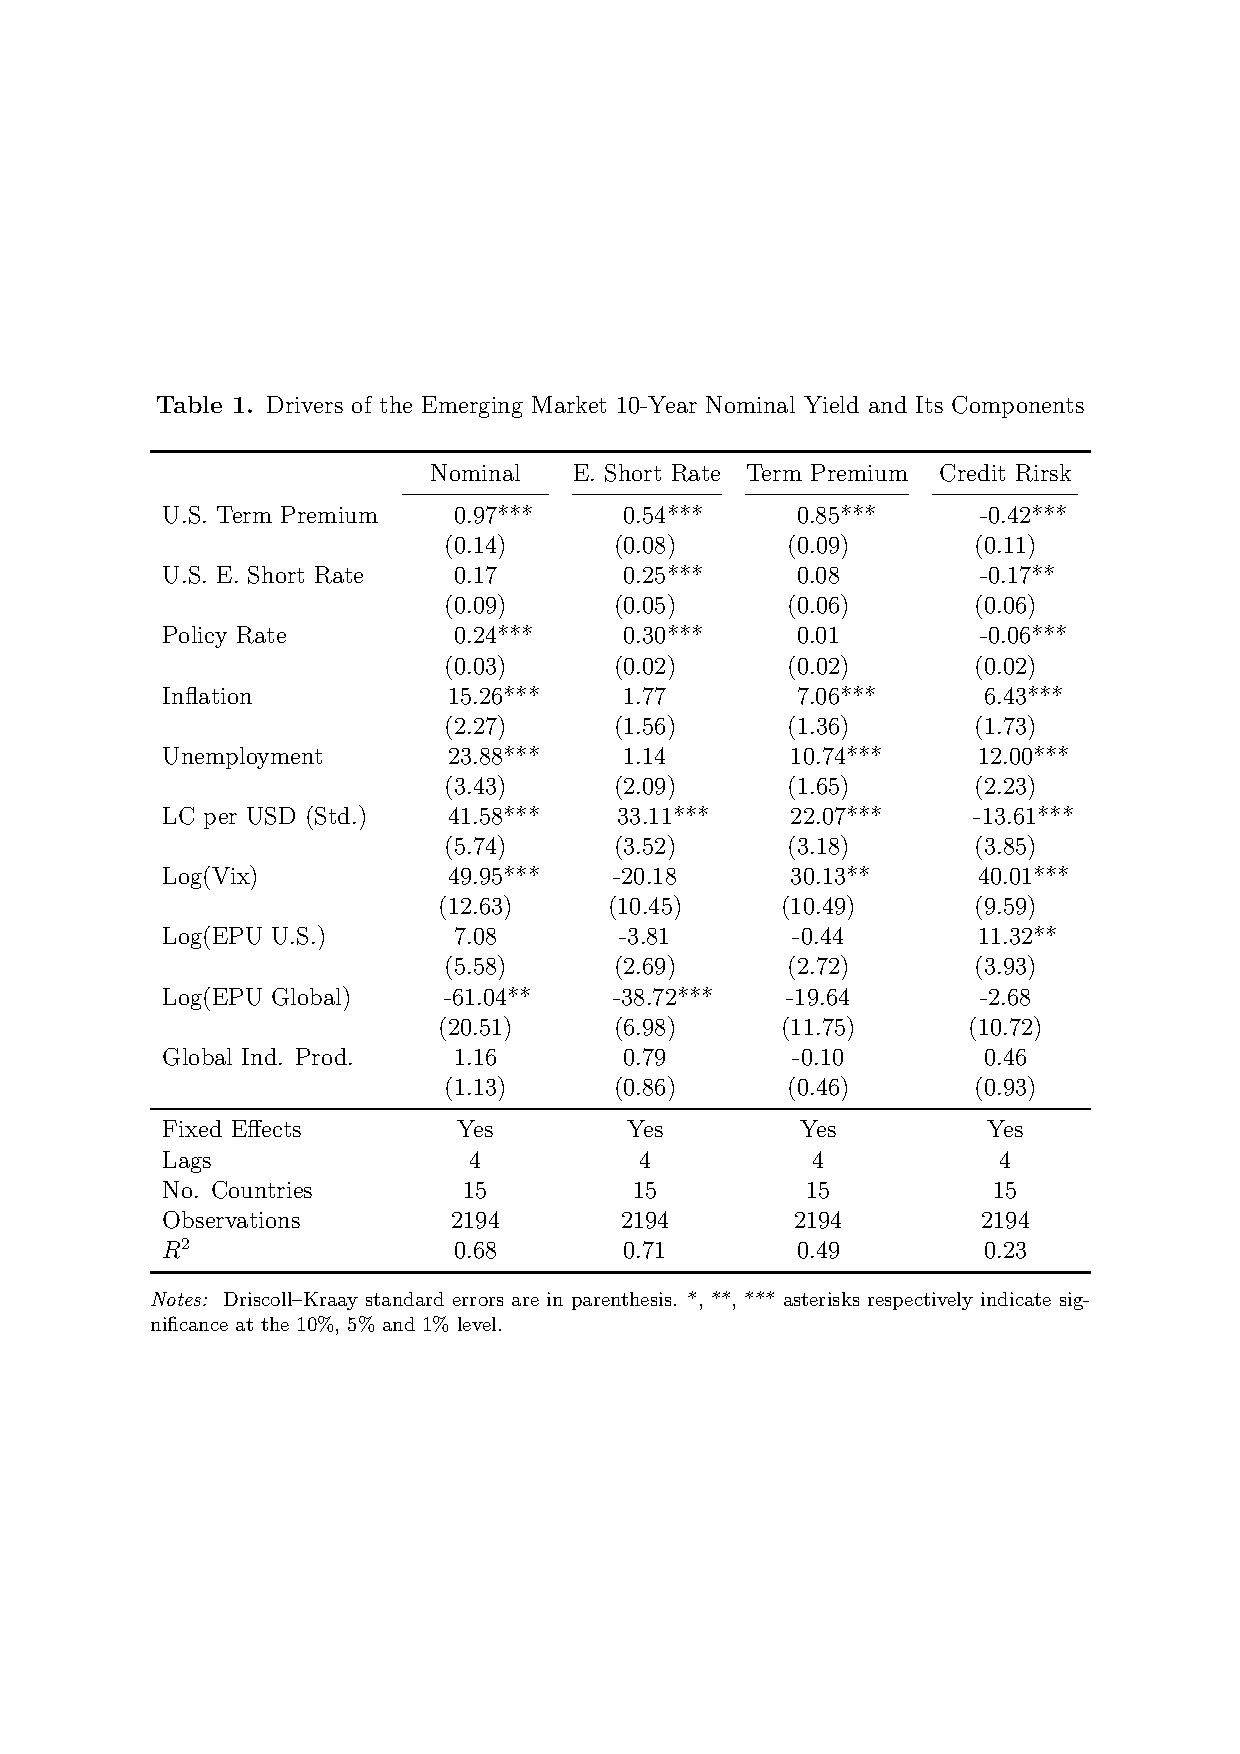
\includegraphics[trim={2cm 7.2cm 2cm 4cm},clip, width=0.95\textwidth,height=1.15\textheight]{../Tables/ycdcmp10y.pdf}
		\par\end{center}
\end{figure}
\begin{textblock*}{5cm}(1.04\textwidth,0.09\textheight)
	\hyperlink{Drivers10Y2Y}{\beamerreturnbutton{10Y \& 2Y}}
\end{textblock*}
\end{frame}


\begin{frame}[label=Drivers2Y]
%	\frametitle{EM Term Premium and Inflation Uncertainty}
\vspace{-0.8cm}
\begin{figure}[!htbp]
\begin{center} % trim removes: left, down, right, top
	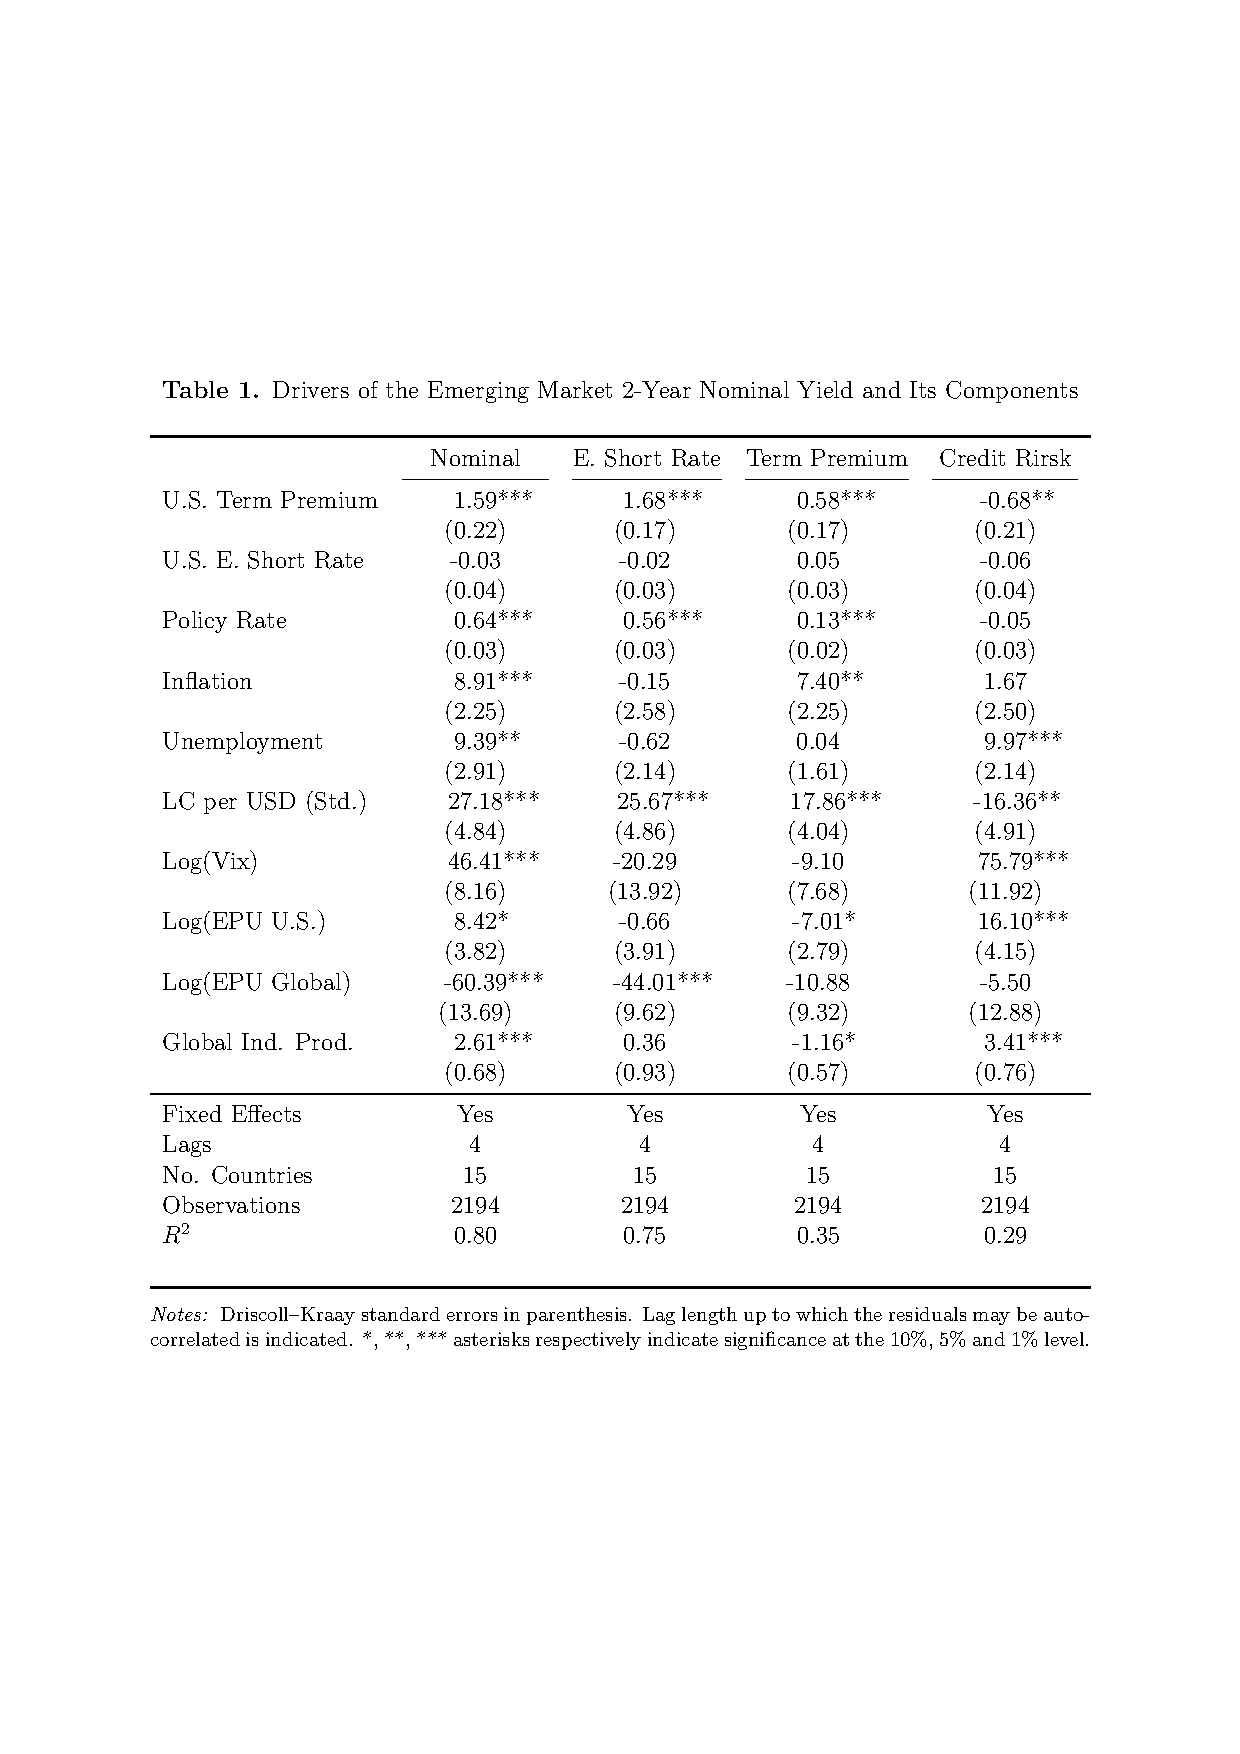
\includegraphics[trim={2cm 7.2cm 2cm 4cm},clip, width=0.95\textwidth,height=1.15\textheight]{../Tables/ycdcmp2y.pdf}
	\par\end{center}
\end{figure}
\begin{textblock*}{5cm}(1.04\textwidth,0.09\textheight)
\hyperlink{Drivers10Y2Y}{\beamerreturnbutton{10Y \& 2Y}}
\end{textblock*}
\end{frame}
\note{monetary autonomy is stronger at the short end than at the long end of the curve}
\note{USTP and GFCy are more relevant for the long end than for the short end of EM YCs}


\begin{frame}[label=TargetUS]
\frametitle{Effects of Target Easing on U.S. Yields}
\begin{figure}[!htbp]
\begin{center} % trim removes: left, down, right, top
\includegraphics[trim={0cm 0cm 0cm 0cm},clip,height=0.45\textheight,width=0.85\linewidth]{../Figures/LPs/LagDep-FX/Target/US/TargetUSDnomyptp120m.eps}
\par\end{center}
\end{figure}
\vspace{-0.5cm}
\begin{figure}[!htbp]
\begin{center} % trim removes: left, down, right, top
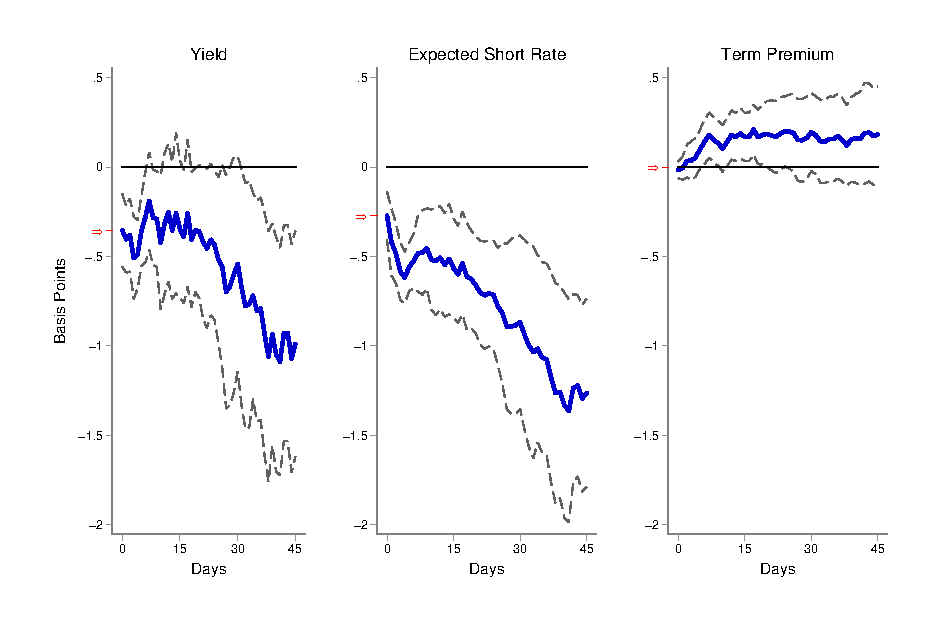
\includegraphics[trim={0cm 0cm 0cm 0.76cm},clip,height=0.45\textheight,width=0.85\linewidth]{../Figures/LPs/LagDep-FX/Target/US/TargetUSDnomyptp24m.eps}
\par\end{center}
\end{figure}
\begin{textblock*}{8mm}(10mm,30mm)
\small \textbf{10Y}
\end{textblock*}
\begin{textblock*}{8mm}(10mm,65mm)
\small \textbf{2Y}
\end{textblock*}
\begin{textblock*}{5cm}(1.07\textwidth,0.65\textheight)
\hyperlink{TargetEM}{\beamerreturnbutton{EM}}
\end{textblock*}
\end{frame}

\begin{frame}[label=FGUSpre]
\frametitle{Effects of Forward Guidance Easing on U.S. Yields: Pre-GFC}
\begin{figure}[!htbp]
	\begin{center} % trim removes: left, down, right, top
		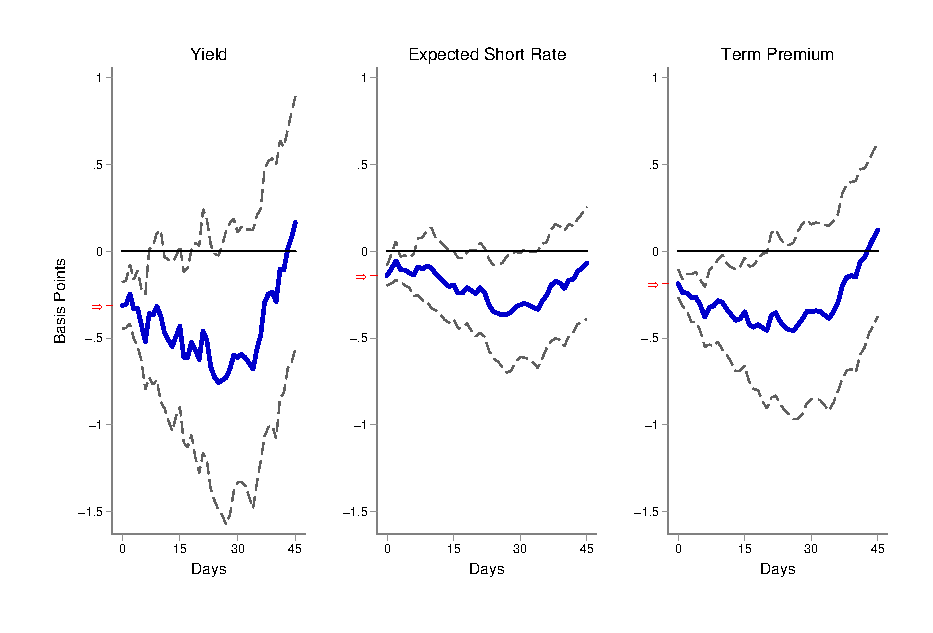
\includegraphics[trim={0cm 0cm 0cm 0cm},clip,height=0.45\textheight,width=0.85\linewidth]{../Figures/LPs/LagDep-FX/Path/US/PathUSDnomyptp120mPre.eps}
		\par\end{center}
\end{figure}
\vspace{-0.5cm}
\begin{figure}[!htbp]
	\begin{center} % trim removes: left, down, right, top
		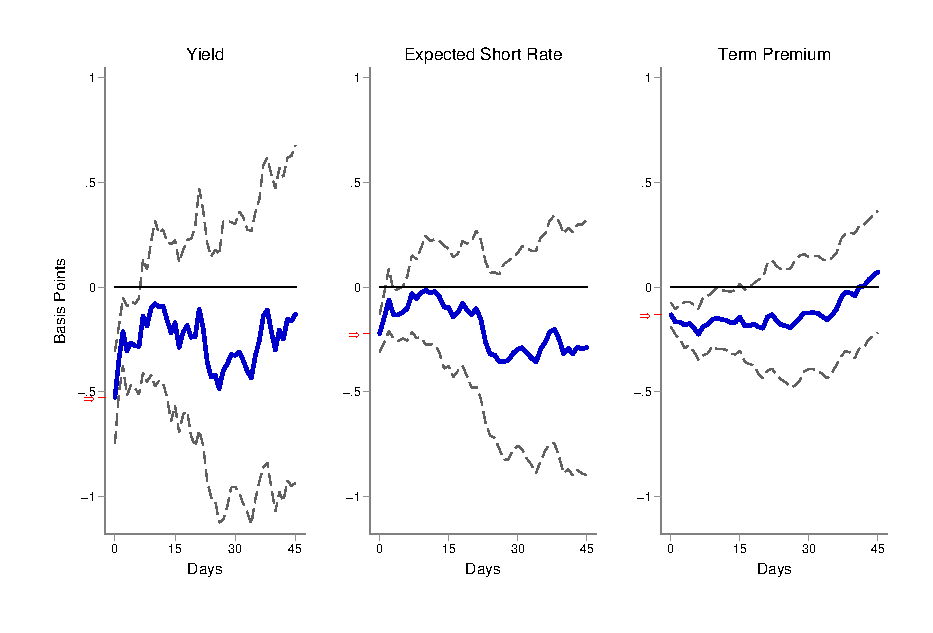
\includegraphics[trim={0cm 0cm 0cm 0.76cm},clip,height=0.45\textheight,width=0.85\linewidth]{../Figures/LPs/LagDep-FX/Path/US/PathUSDnomyptp24mPre.eps}
		\par\end{center}
\end{figure}
\begin{textblock*}{8mm}(10mm,30mm)
	\small \textbf{10Y}
\end{textblock*}
\begin{textblock*}{8mm}(10mm,65mm)
	\small \textbf{2Y}
\end{textblock*}
\begin{textblock*}{5cm}(1.07\textwidth,0.65\textheight)
	\hyperlink{FGEMpre}{\beamerreturnbutton{EM}}
\end{textblock*}
\end{frame}

\begin{frame}[label=FGUSpost]
\frametitle{Effects of Forward Guidance Easing on U.S. Yields: Post-GFC}
\begin{figure}[!htbp]
\begin{center} % trim removes: left, down, right, top
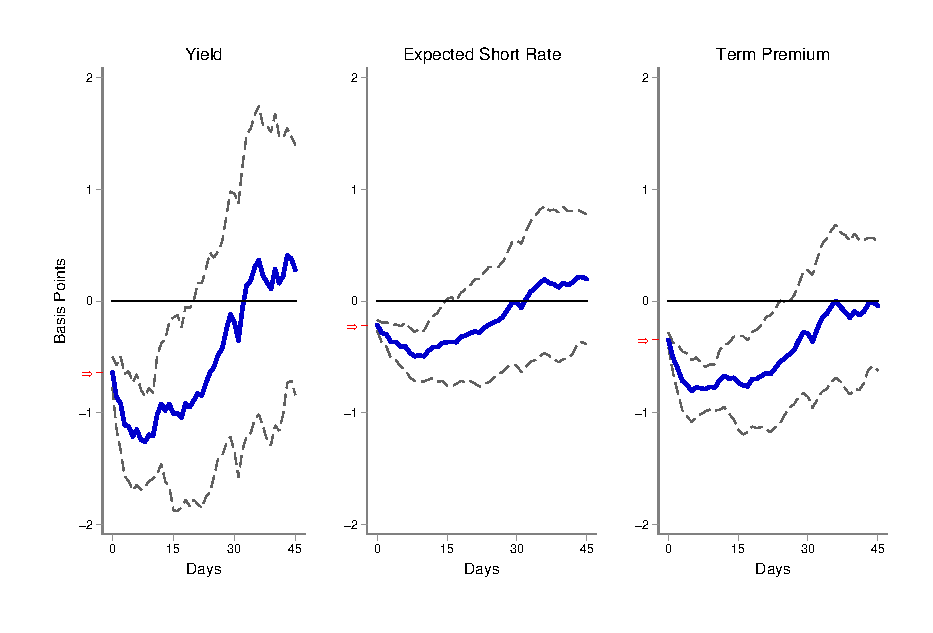
\includegraphics[trim={0cm 0cm 0cm 0cm},clip,height=0.45\textheight,width=0.85\linewidth]{../Figures/LPs/LagDep-FX/Path/US/PathUSDnomyptp120mPost.eps}
\par\end{center}
\end{figure}
\vspace{-0.5cm}
\begin{figure}[!htbp]
\begin{center} % trim removes: left, down, right, top
\includegraphics[trim={0cm 0cm 0cm 0.76cm},clip,height=0.45\textheight,width=0.85\linewidth]{../Figures/LPs/LagDep-FX/Path/US/PathUSDnomyptp24mPost.eps}
\par\end{center}
\end{figure}
\begin{textblock*}{8mm}(10mm,30mm)
\small \textbf{10Y}
\end{textblock*}
\begin{textblock*}{8mm}(10mm,65mm)
\small \textbf{2Y}
\end{textblock*}
\begin{textblock*}{5cm}(1.07\textwidth,0.65\textheight)
\hyperlink{FGEMpost}{\beamerreturnbutton{EM}}
\end{textblock*}
\end{frame}

\begin{frame}[label=LSAPUS]
\frametitle{Effects of Asset Purchase Easing on U.S. Yields}
\begin{figure}[!htbp]
\begin{center} % trim removes: left, down, right, top
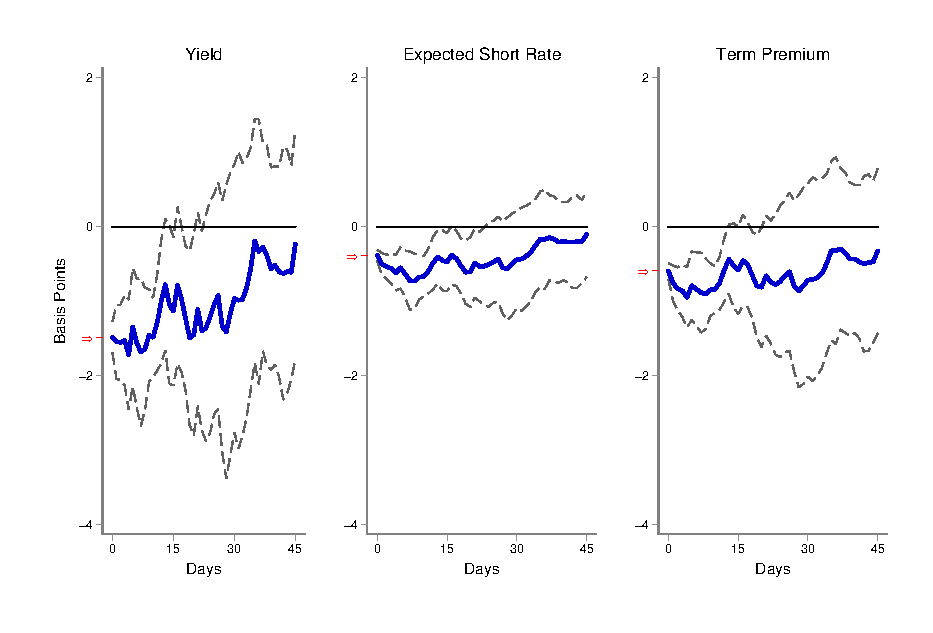
\includegraphics[trim={0cm 0cm 0cm 0cm},clip,height=0.45\textheight,width=0.85\linewidth]{../Figures/LPs/LagDep-FX/LSAP/US/LSAPUSDnomyptp120m.eps}
\par\end{center}
\end{figure}
\vspace{-0.5cm}
\begin{figure}[!htbp]
\begin{center} % trim removes: left, down, right, top
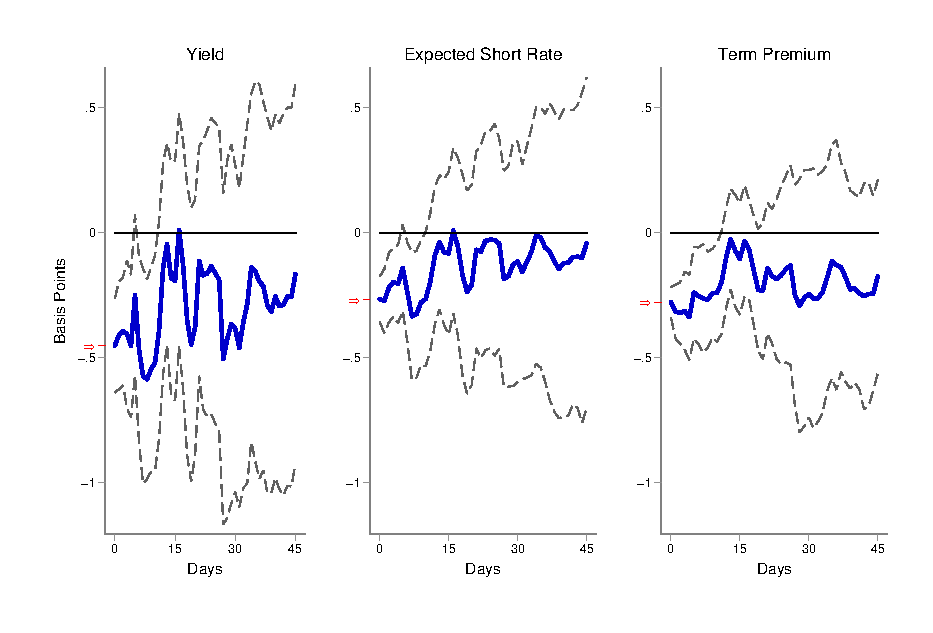
\includegraphics[trim={0cm 0cm 0cm 0.76cm},clip,height=0.45\textheight,width=0.85\linewidth]{../Figures/LPs/LagDep-FX/LSAP/US/LSAPUSDnomyptp24m.eps}
\par\end{center}
\end{figure}
\begin{textblock*}{8mm}(10mm,30mm)
\small \textbf{10Y}
\end{textblock*}
\begin{textblock*}{8mm}(10mm,65mm)
\small \textbf{2Y}
\end{textblock*}
\begin{textblock*}{5cm}(1.07\textwidth,0.65\textheight)
\hyperlink{LSAPEM}{\beamerreturnbutton{EM}}
\end{textblock*}
\end{frame}

%---------------------------------------------------------------
% Sources
%---------------------------------------------------------------
% Tips in general
% https://en.wikibooks.org/wiki/LaTeX/Presentations
%https://tex.stackexchange.com/questions/12328/how-can-i-use-todonotes-with-beamer
% Insert links to slides
% https://latex.org/forum/viewtopic.php?t=4594
% Place button of link on slide
%https://tex.stackexchange.com/questions/50643/hyperlink-button-in-an-exact-position
% Make figures visible
%https://stackoverflow.com/questions/4683093/beamer-how-to-show-images-as-step-by-step-images
% Multicolumn and multirow
%https://tex.stackexchange.com/questions/156219/proper-centering-with-cmidrule-and-multi-row-and-column

% Metropolis
%http://mirrors.ibiblio.org/CTAN/macros/latex/contrib/beamer-contrib/themes/metropolis/doc/metropolistheme.pdf
%https://github.com/matze/mtheme

% Code for hyperlinks
%[label=corr_10yr]
%\begin{textblock*}{3cm}(.9\textwidth,-.5\textheight)
%	\hyperlink{corr_10yr}{\beamergotobutton{10-Year TP}}
%\end{textblock*}
%
%\begin{textblock*}{3cm}(.9\textwidth,-.5\textheight)
%	\hyperlink{corr_10yr}{\beamerreturnbutton{10-Year TP}}
%\end{textblock*}

% Two-column frame template
%http://felix11h.github.io/blog/beamer-two-col



%\begin{frame}[allowframebreaks]{References}
\begin{frame}<presentation:0>
\bibliographystyle{abbrvnat} 
\bibliography{../../../References/library}
\end{frame}

\end{document}